\chapter[Electron and Proton Acceleration in Transrelativistic Magnetic Reconnection: Dependence on $\sigma$ and $\beta$]
{Electron and Proton Acceleration in Transrelativistic Magnetic Reconnection: Dependence on $\sigma$ and $\beta$}
\section{Introduction}
%Low-luminosity accretion flows, such as the one at the center of the Milky Way, Sagittarius A* (Sgr A*), are well described by a ``radiatively inefficient accretion flow'' (RIAF).  RIAFs are geometrically thick and optically thin, consisting of a relatively dilute and hot plasma.  Because of the low densities in these disks, the timescale for Coulomb collisions between particles is extremely long, permitting the plasma to exist in a two-temperature state, where the ions and electrons are thermally decoupled.  Additionally, because collisions are so rare, the particle distribution functions are likely to have a significant non-thermal component, which can be generated by various acceleration mechanisms such as shocks, magnetic reconnection, and the dissipation of turbulence.  Non-thermal particle acceleration associated with these plasma processes can only be described in a fully-kinetic framework, and hence are well suited to study via particle-in-cell (PIC) simulations.  The results from PIC simulations can provide subgrid models for magneto-hydrodynamic simulations, in order to account for physics that is not captured in standard fluid theories.

%In \citet{ball2016}, we showed that a localized population of highly energetic non-thermal electrons in a radiatively inefficient accretion flow can generate significant x-ray variability that purely thermal MHD models are unable to reproduce.  Motivated by this study, in \citet{ball2017}, we characterized the properties of current sheets in general-relativistic magneto-hydrodynamic simulations of radiatively inefficient accretion flows, and found that the typical magnetization $\sigma$ of the current sheets are in the trans-relativistic regime $\sigma \approx 1$.  


One of the key parameters that determines the outcome of reconnection and the properties of the resulting particle distribution is the  magnetization of the ambient plasma, i.e., the ratio $\sigma$ of magnetic energy density to enthalpy density. 
%expressed by the parameter $\sigma=B_{0}^{2}/4\pi w_{0}$, where $B_{0}$ is the magnetic field strength in the ambient plasma, and $w_{0}$ is the initial enthalpy density.  
Numerous studies have investigated the non-relativistic ($\sigma\ll 1$) regime, which has applications to the solar corona and solar flares (e.g., \citealt{drake2013}; \citealt{dahlin2014}; \citealt{shay2014}; \citealt{liguo2015}).  The ultra-relativistic ($\sigma\gg 1$) regime has also been explored in detail, due to its relevance to high-energy emission from blazar jets and pulsar wind nebulae (e.g., \citealt{kagan2013}; \citealt{sironi2014}; \citealt{guod_14, guo2015, guo_16}; \citealt{melzani2014}; \citealt{kagan2015}; \citealt{nalewajko2015}; \citealt{werner2016}; \citealt{sironi2016}).  However, only a limited number of studies have been carried out in the trans-relativistic regime ($\sigma \sim 1$), addressing particle heating (\citealt{rowan2017}) and acceleration (\citealt{melzani2014b}; \citealt{werner2018}). The trans-relativistic regime is of particular interest to studies of radiatively inefficient accretion flows around black holes, such as Sgr A* at our Galactic center. Here, current sheets with typical magnetizations of $\sigma\sim1$ are frequently observed in global MHD simulations (\citealt{ball2017}).  Localized particle acceleration powered by magnetic reconnection in these settings could give rise to high-energy variability (\citealt{ball2016}; \citealt{li2017}).  

Earlier investigations (e.g., \citealt{schoeffler2011}; \citealt{schoeffler2013}; \citealt{rowan2017}) have shown that, in addition to the magnetization $\sigma$, the initial plasma temperature, or equivalently the proton $\beta$ (i.e., the ratio of proton thermal pressure to magnetic pressure), can affect the dynamics and energetics of magnetic reconnection.  In particular, \citet{rowan2017} explored the dependence of the electron and proton heating efficiency on the magnetization $\sigma$, the proton $\beta$, and the electron-to-proton temperature ratio.  However, the role of $\beta$ on non-thermal particle acceleration in the trans-relativistic regime ($\sigma\sim1$) remains largely unexplored. 

The works by \citet{melzani2014b} and \citet{melzani2014} were the first to investigate particle acceleration in the trans-relativistic regime of reconnection. They examined the energy partition between protons and electrons and the electron power-law spectra, but they employed a reduced proton-to-electron mass ratio, and they only explored a relatively narrow range of $\beta$. \citet{werner2018} performed an extensive study across a wide range of $\sigma$, from the trans-relativistic through the ultra-relativistic regime, and reported how the reconnection rate, the electron power-law slope, and the energy partition between electrons and protons depend on $\sigma$.  They found that the electron power-law slope decreases with increasing $\sigma$ (so, the spectrum hardens) and provided an empirical fit $p\simeq1.9+0.7/\sqrt{\sigma}$ for the power-law slope $p$ of the electron spectrum.  However, their study was performed at a fixed value of proton beta $\beta=0.01$.  

 %This study is the first to systematically map out the details of particle acceleration in the transition from the trans-relativistic to the ultra-relativistic regimes.  


%Given the importance of $\sigma$ and the plasma-$\beta$ in the outcome of particle acceleration and heating from magnetic reconnection, PIC studies aim to map out the dependence of the final particle energy spectra across this parameter space. 
In this work, we investigate proton and electron non-thermal acceleration in trans-relativistic  reconnection, covering the whole parameter space in $\sigma$ and $\beta$ and employing the physical proton-to-electron mass ratio. For four values of the magnetization ($\sigma=$ 0.1, 0.3, 1, and 3), we explore a wide range of $\beta$, from $\beta=10^{-4}$ up to the maximum possible value of $\beta$, that is $\beta_{\rm max}\approx 1/4\sigma$ (we will discuss why this is the maximum in Section \ref{setup}). Our study goes beyond the current state of the art in several respects: we explore for the first time the dependence of the non-thermal electron spectrum on  plasma $\beta$, and we examine the role of various electron acceleration mechanisms, by tracking particles in our simulations. In addition, our computational domains are larger than previous works by at least a factor of $\sim5$.
While we primarily focus on electrons, we also present proton spectra and briefly investigate proton acceleration mechanisms.

We find that the electron spectrum in the reconnection region can be generally modeled as a non-thermal power law, but the properties of the spectrum are strongly dependent on $\beta$. At $\beta \lesssim 3 \times 10^{-3}$, the spectrum is dominated by a hard power law, whose slope is insensitive to $\beta$ and depends on $\sigma$ as $p\simeq 1.8 +0.7/\sqrt{\sigma}$, in agreement with the result by \citet{werner2018}. The electron spectrum tends to steepen for larger simulation domains. Electrons are primarily accelerated by the non-ideal electric field at X-points, either  in the initial current layer  or in current sheets generated in between merging magnetic islands. 
At higher $\beta$, the electron power law steepens significantly, and the electron spectrum eventually approaches a Maxwellian distribution, for all values of $\sigma$. At high values of $\beta$ near $\beta_{\rm max}\approx1/4\sigma$, when both electrons and protons start relativistically hot, the spectrum of both species displays an additional component at high energies, containing a few percent of particles, which are accelerated via a Fermi-like process by bouncing in between the reconnection outflow and the stationary magnetic island at the boundary of our periodic domain.
We investigate the dependence of our results on the size of the simulation domain, finding that  the high-energy  cutoff of the electron spectrum increases with box size. 
For the main population of non-thermal electrons (i.e., excluding the additional component emerging at $\beta\rightarrow \beta_{\rm max}$),
we provide an empirical prescription for the dependence of the power-law slope and the acceleration efficiency on $\beta$ and $\sigma$. The results of our study can be used as subgrid models in global MHD simulations of  black hole accretion flows (e.g., \citealt{ball2016}; \citealt{mao2017}; \citealt{chael2017}), potentially unveiling the origin of the flaring behaviour of Sgr A* \citep{ponti17}.

The layout of the paper is as follows.  In Section \ref{setup} we describe the setup of our simulations.  In Section \ref{time_evol}, we show and describe the time evolution of a representative simulation and the evolution of its associated electron and proton energy spectra.  In Section \ref{role_of_beta}, we explore the dynamics of the reconnection layer as a function of $\sigma$ and $\beta$, and illustrate the key differences between low- and high-$\beta$ reconnection.  In Section \ref{energy_spectra}, we show the electron and proton spectra for a number of values of $\sigma$ and $\beta$, and provide an empirical fit to the electron power-law slopes and acceleration efficiencies.  Finally, in Section \ref{mechanism}, we show representative trajectories of accelerated electrons for both a low-$\beta$ and a high-$\beta$ simulation.  We conclude and summarize in Section \ref{conclusions}.

\section{Simulation Setup}\label{setup}
We perform a large suite of PIC simulations of anti-parallel magnetic reconnection using the  publicly-available code TRISTAN-MP (\citealt{buneman93}; \citealt{spitkovsky05}).  We employ a two-dimensional (2D) simulation domain in the $xy$ plane, but we track all three components of velocity and electromagnetic field vectors.  We set up the system in Harris equilibrium, with a magnetic field profile $\bm{{B}} = -B_{0}\tanh{\left(2\pi y / \Delta\right)}\bm{\hat{x}}$, where $B_{0}$ is the strength of the reconnecting field in the ambient plasma and $\Delta$ is the thickness of the sheet.  $B_{0}$ is related to the magnetization parameter $\sigma$ via $\sigma=B_{0}^2 / 4\pi w_{0} $, where $w_{0}$ is the enthalpy density of the ambient plasma $w_0=(\rho_{e}+\rho_{i})c^{2}+ \hat{\gamma}_{e}u_{e}+ \hat{\gamma}_{i}u_{i}$, with $\rho_{i,e}$, $\hat{\gamma}_{i,e}$, and $u_{i,e}$ being the mass densities, adiabatic indices, and internal energy densities of ambient protons and electrons, respectively.  The temperature is specified through the proton $\beta$, defined as $\beta \equiv \beta_{i}=8 \pi n_{i} k T_{i}/B_{0}^{2}$, where $n_i=\rho_i/m_i$ is the proton number density, $T_i$ is the proton temperature, and $m_i$ is the proton mass. Ambient electrons and protons start with the same temperature, so $\beta_e=\beta_i=\beta$ (the total plasma beta, including both species, is $2\,\beta$). In most cases, the ambient protons are non-relativistic, so the magnetization parameter as defined with the proton rest mass $\sigma_i=B_0^2/4\pi \rho_i c^2$ is nearly identical to the enthalpy-weighted magnetization $\sigma$ defined above. Each computational cell in the ambient plasma is initialized with four particles per cell (so, $N_{ppc}=4$), but we have tested that our results are the same when using $N_{ppc}=16$ (see Appendix \ref{convergence}).

The thickness of the current sheet is $\Delta = 80 \,c/\omega_{p}$, where $\omega_{p}$ is the electron plasma frequency, given by 

\begin{equation}
\omega_{p} =\sqrt{\frac{4\pi n_{e}e^{2}}{m_{e}}}\left(1+\frac{\theta_{e}}{\hat{\gamma_{e}}-1}\right)^{-1/2}.
\label{electron skin depth}
\end{equation}
Here, $e$ is the electron charge, $m_e$ is the electron mass, $n_e=\rho_e/m_e$ is the electron number density ($=n_i$) and $\theta_{e}$ is the dimensionless electron temperature $\theta_{e}=kT_{e}/m_{e}c^{2}$ in the ambient plasma. 
We set up the initial Harris equilibrium by initializing the plasma in the current sheet to be hot and overdense (by a factor of 3 with respect to the background) so that its thermal pressure balances the magnetic pressure outside the sheet. The particles in the current sheet are set up as a Maxwellian distribution drifting in the $z$ direction, so that their electric current balances the curl of the magnetic field. 

Our computational domain is periodic in the $x$-direction of the reconnection outflow (in order to retain all accelerated particles), while the box is continually enlarged in the $y$-direction, as two moving injectors --- that steadily inject magnetized plasma into the simulation domain --- recede from the current sheet at the speed of light along $\pm\bm{\hat{y}}$. By employing the moving injectors and a dynamically-enlarging box (see \citealt{sironi2009} for further details), we can study the late-time evolution of the system without being artificially limited by the finite amount of plasma and magnetic flux that is initially in the simulation domain. Additional computational optimization is achieved by allowing the injectors to periodically ``jump'' back towards the current sheet, removing all particles beyond the injectors and resetting the electromagnetic fields to their initial values.

The length of the box in the $x$ direction of the reconnection outflow is $L_x=16620$ cells, which corresponds to $L_x\simeq5540\,c/\omega_{p}$, since we resolve the electron skin depth $c/\omega_{p}$ with 3 computational cells. As described in Appendix \ref{convergence}, we have tested that our results are the same when the electron skin depth is resolved with 6 cells. We also investigate the dependence of our results on the extent $L_x$ of the computational domain (up to a factor of two larger than our reference runs), see Appendix \ref{boxsize}.

We trigger reconnection in the center of the box by removing by hand the pressure of the hot particles initialized in the center of the sheet (see \citealt{sironi2016}).  This causes the current sheet to collapse and form two ``reconnection fronts,'' which are pulled by magnetic tension along $\pm \bm{\hat{x}}$ at roughly the Alfv\'en speed $v_{A}=c\sqrt{\sigma/(1+\sigma)}$.  We define the Alfv\'enic crossing time as  $t_{A} = L_{x}/v_{A}$.  At $t\gtrsim 0.5\,t_A$, the reconnected plasma starts accumulating at the boundary of the periodic simulation domain, where a ``boundary island'' forms.

Astrophysical current sheets are likely thick, making the timescale for spontaneous (or ``untriggered'') reconnection very long compared to relevant dynamical timescales.  This means that astrophysical reconnection is likely triggered by some large-scale perturbation, which motivates our decision to trigger reconnection in our simulations. In fact, the large-scale perturbation will induce a curvature of the field lines over a scale $\sim L_x$, such that the current sheet is narrower near the center. The central region is then most likely to go unstable via the tearing mode, and the signal of ongoing reconnection will propagate toward the outer regions (where the current sheet is broader) before they have time to spontaneously become unstable. We further discuss our choice of a triggered setup in  Appendix \ref{untriggered}, where we compare our results to the case of untriggered reconnection, where the  system goes unstable via numerical noise, as in \citealt{sironi2014}. In Appendix \ref{untriggered}, we also compare the results of triggered simulations with either periodic or outflow boundaries in the $x$ direction (for further details on the implementation of the outflow boundary conditions, see \citealt{sironi2016}).


\begin{deluxetable}{ccccccc}
\centering
\tablewidth{1\columnwidth}
\tablecaption{Simulation Parameters}  
\tablehead{run&$\sigma$& $\sigma_{i}$ & $\beta$ & $L_{x}$ ($c/\omega_{pi}$) &$L_{x}$ ($r_{e,\rm hot}$) &$kT_{i}/m_{i}c^{2}$}
\startdata
A0& 0.1 & 0.1& $1\times 10^{-4}$ & 125 & 406&$5 \times 10^{-6}$\\ 
 \hline
A1& 0.1 & 0.1& $3\times 10^{-4}$ & 127 & 417&$1.5 \times 10^{-5}$\\ 
 \hline
A2& 0.1& 0.1 & $10^{-3}$ & 134& 453 & $5 \times 10^{-5}$\\
 \hline
A3& 0.1& 0.1 & $3\times 10^{-3}$ & 158 & 542 & $1.5 \times 10^{-4}$\\
 \hline
A4& 0.1& 0.1 & 0.01  & 233& 776 & $5 \times 10^{-4}$\\
 \hline
A5&  0.1 & 0.1& 0.02& 312 & 1020& $1 \times 10^{-3}$\\
 \hline
A6&  0.1 &  0.1 &0.1 & 664& 2110 & $5 \times 10^{-3}$\\
 \hline
A7 & 0.1& 0.11 & 0.3 & 1138 & 3978& 0.02\\
 \hline
A8& 0.1 &0.16& 1.5  & 4133& 7269 & 0.1\\ %[1ex] 
 \hline
B0 & 0.3&0.3 & $1\times 10^{-4}$ & 127& 241&$1.5\times 10^{-5}$\\ 
 \hline
B1 & 0.3&0.3 & $3\times 10^{-4}$  & 134& 261&$5\times 10^{-5}$\\ 
 \hline
B2& 0.3&0.3 & $10^{-3}$  & 156& 313&$1.5\times 10^{-4}$\\
  \hline
B3& 0.3&0.3 & $3\times 10^{-3}$ & 232& 448&$5\times 10^{-4}$\\
 \hline
B4& 0.3&0.3 & $6\times 10^{-3}$ &312& 589 &$1\times 10^{-3}$\\
 \hline
B5& 0.3&0.3 & 0.01 &375& 701&$1.5\times 10^{-3}$\\
 \hline
B6&  0.3&0.3 & 0.03 & 664& 1218&$5\times 10^{-3}$\\
 \hline
B7&  0.3 & 0.34&0.11 & 1138& 2296&0.02\\
 \hline
B8*& 0.3&0.72 & 0.55 & 4133& 4956&0.2\\ %[1ex] 
 \hline
C0&  1 &1& $1\times 10^{-4}$ & 134& 143&$5 \times 10^{-5}$\\ 
 \hline
C1&  1 &1& $3\times 10^{-4}$ & 157& 171&$1.5 \times 10^{-4}$\\ 
 \hline
C2& 1 &1& $10^{-3}$  &232& 245&$5 \times 10^{-4}$\\
 \hline
C3& 1 &1& $3\times 10^{-3}$ & 375& 384&$1.5 \times 10^{-3}$\\
 \hline
C4& 1 &1& 0.01 & 664& 667&$5 \times 10^{-3}$\\
 \hline
C5& 1&1.1 & 0.03 & 1138& 1107& 0.015\\
 \hline
C6& 1&1.3 & 0.08  & 2069& 1827& 0.05\\
 \hline
C7*& 1&2.4 & 0.16 & 4133& 2713&0.2\\
  \hline
D0&  3&3 & $10^{-4}$ & 157& 99 & $1.5 \times 10^{-4}$\\ 
 \hline
D1& 3 &3& $3\times 10^{-4}$ & 232& 141& $5 \times 10^{-4}$\\ 
 \hline
D2& 3 &3& $10^{-3}$ & 375& 221& $1.5 \times 10^{-3}$\\
 \hline
D3& 3 &3.1& $3\times 10^{-3}$ & 664& 385& $5 \times 10^{-3}$\\
 \hline
D4& 3&3.3 & 0.01 & 1138& 639&0.015\\
 \hline
D5*&  3&4.0 & 0.026 & 2069& 1055&0.05\\
 \hline
D6*&  3 &7.2 &0.055  & 4133& 1566&0.2
  %\hline
\enddata
\tablecomments{Summary of the physical and numerical parameters of our simulations.  All simulations are performed with the physical mass ratio, equal electron and proton temperatures, a resolution of 3 cells per electron skin depth, and 5,440 electron skin depths along the current layer.}
\label{tab:fit}
\end{deluxetable}

The physical and numerical parameters of our simulations are summarized in Table 1. To fully map out the parameter space of interest, we perform 33 simulations across four different values of the magnetization: $\sigma=\,$0.1, 0.3, 1, and 3. For each value of $\sigma$, we have multiple (at least 7) simulations in which we vary the proton $\beta$ from $10^{-4}$ up to the maximum possible value of $\beta$, $\beta_{\rm max}\approx 1/4\sigma$. This upper limit in $\beta$ is reached when both protons and electrons become relativistically hot. In this limit, the internal energy densities dominate over the rest mass energy densities, so the enthalpy density is  $w_0\simeq \hat{\gamma}_{e}u_{e}+\hat{\gamma_{i}}u_{i}$. For $\hat{\gamma}_{e}=\hat{\gamma}_{i}=4/3$, as appropriate for a 3D ultra-relativistic gas, the magnetization tends to $\sigma \simeq 1/4\beta$, which defines an upper limit on $\beta$ at a given $\sigma$, equal to $\beta_{\rm max}\approx 1/4\sigma$.


Due to computational constraints, PIC codes often employ a reduced proton-to-electron mass ratio, in order to decrease the separation of scales between the two species. However, as we have shown in  \citealt{rowan2017}, a choice of the mass ratio smaller than the physical one can artificially affect the partition of energy between electrons and protons in trans-relativistic reconnection. Since it could also artificially affect the efficiency and slope of non-thermal particle acceleration, in this study we employ the physical mass ratio $m_{i}/m_{e}=1836$. While the box length $L_x$ measured in electron skin depths is independent of $\beta$ or $\sigma$, the box length in proton skin depths $c/\omega_{pi}$, where
$$
\omega_{pi} =\sqrt{\frac{4\pi n_{i}e^{2}}{m_{i}}}\left(1+\frac{\theta_{i}}{\hat{\gamma_{i}}-1}\right)^{-1/2},
$$ 
varies significantly with $\beta$ due to the $\theta_e$-dependent correction in Equation \ref{electron skin depth}.  For most of our simulations, electrons start as ultra-relativistically hot, while protons are non-relativistic (our maximum $\theta_{i}=kT_i/m_i c^2$ is 0.2, see Table 1).  As  $\beta$ increases, the separation of electron and proton scales decreases, so our domain is effectively larger (in units of the proton skin depth) at higher $\beta$ (see Table 1). In Table 1, we also quote the extent of our simulation domain in units of $r_{e,\rm hot}=\sigma_e m_e c^2/eB_0$ (the unit of length employed by \citealt{werner2018}), which corresponds to the Larmor radius of a relativistic electron with Lorentz factor $\sigma_e=\sigma_i m_i/m_e$.



\begin{figure}[!h]
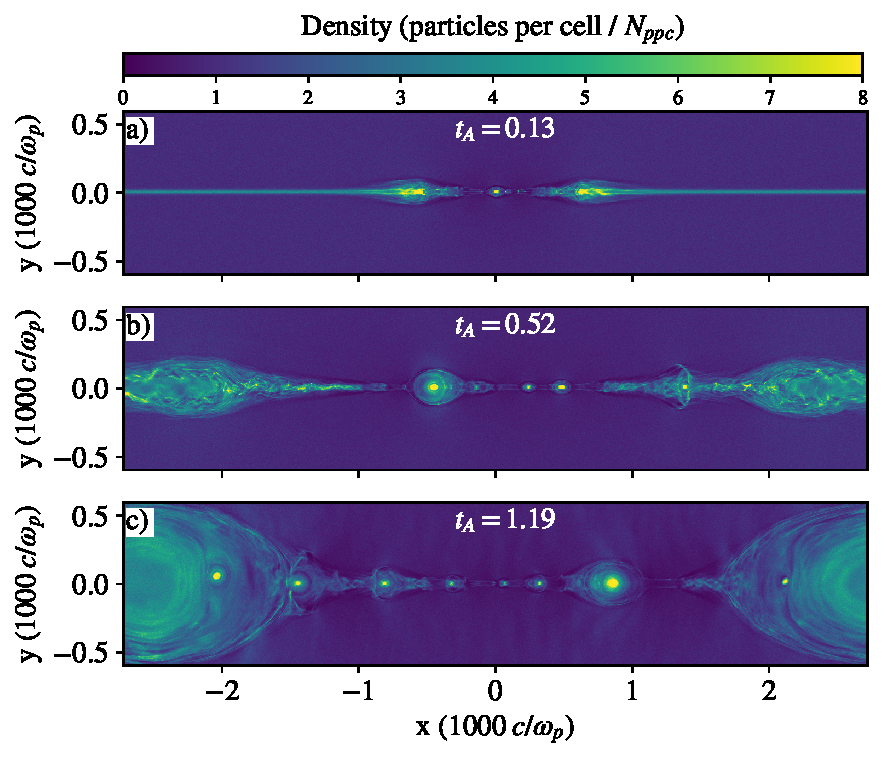
\includegraphics[width=1.0\linewidth]{testing_threeplot.pdf}
\caption{2D snapshots of density depicting the time evolution from a simulation with $\sigma=0.3$ and $\beta=3\times 10^{-4}$ (run B1) at three different times.  The top, middle, and bottom panels correspond to 0.13, 0.52, and 1.19 Alfv\'en crossing times, respectively.  We normalize the density to the initial number of particles per cell in the ambient plasma, $N_{ppc}$.  We scale the density to the power of $0.3$ to enhance the contrast in color scale.}
\label{lowbeta_threeplot}
\end{figure}

\section{Time Evolution of the reconnection layer}\label{time_evol}
In order to illustrate the time evolution of a typical simulation, we show in Figure \ref{lowbeta_threeplot} a series of 2D snapshots of the particle number density for a run with $\sigma=0.3$ and $\beta=3\times10^{-4}$. The lack of pressure support in the vicinity of the center, resulting from our initial perturbation, triggers the collapse of the current sheet (top panel in Figure \ref{lowbeta_threeplot}) and the formation of an X-point. In the following, we shall indicate this X-point as the ``primary X-point.'' While in untriggered systems the tearing mode instability pinches the current sheet at several locations, thus producing several primary X-points, in our triggered setup we only have one primary X-point. The top panel also shows the two reconnection fronts (at $x \approx \pm 500\, c/\omega_{p}$) that are pulled towards the edges of the box by the tension of the magnetic field lines.  In the underdense region in between these fronts, a secondary plasmoid begins to form close to the center, as plasma flows in from above and below the  reconnection layer.  

In the middle panel of Figure \ref{lowbeta_threeplot}, the reconnection fronts are approaching the edges of the box, and numerous secondary plasmoids have formed in the layer, separated by secondary X-points (see e.g., \citealt{loureiro2007}; \citealt{uzdensky2010}; \citealt{huang2012}; \citealt{takamoto2013} and \citealt{comisso2016} for the physics of secondary plasmoid formation).  By ``secondary plasmoids,'' we are referring to structures that form after the early collapse of the current sheet, and that contain particles that belong to the ambient plasma (as opposed to the hot population of particles initialized in the current sheet). A secondary X-point is present in between each pair of neighboring secondary plasmoids. 
The largest plasmoid near the center of the box, at $x\simeq-300 \; c/\omega_{p}$, is formed via mergers of several smaller plasmoids, and contains the highest energy particles in the system at this time (see \citealt{sironi2016} for a discussion of the correlation between plasmoid size and  maximum particle energy).  

In the final snapshot (bottom panel in Figure \ref{lowbeta_threeplot}), the outflowing fronts collide across the periodic boundaries, forming a large magnetic island which sits passively at the edge and acts as a reservoir for accelerated particles. In the following, we shall refer to this structure as the ``boundary island,'' and by ``plasmoids'' we will only mean secondary islands. Secondary plasmoids forming in the sheet are eventually advected into the boundary island by the  tension of the field lines.   A current sheet forms at the interface between the boundary island and each secondary plasmoid that is merging into it. As we will show in Section \ref{mechanism}, this interface is a site of efficient electron acceleration.




\subsection{Defining the Reconnection Region}
The spectrum from the entire simulation domain includes both pre- and post-reconnection plasma.  Because of this, it is prudent to have a scheme to distinguish between particles that have undergone reconnection, and particles that are still in the colder upstream region.  This is an important step to correctly interpret the spectra, and avoid mistaking for a power-law component the ``bridge'' between the pre- and post-reconnection distributions.
In order to extract the spectrum of the plasma that has undergone reconnection, uncontaminated by the cold upstream plasma, we use a mixing criterion to identify regions where reconnection has occurred (as first proposed in \citealt{daughton2014}, and described in \citet{rowan2017}).  In short, we tag particles with an identifier that specifies whether they were initialized above or below the current sheet.  We can then identify the cells where particles have mixed to a sufficient degree and in doing so, define the ``reconnection region'', predominantly populated by particles that have been processed by reconnection.   We take a mixing fraction of one part in 100 as our lower limit to define this region.  Using this technique, we are able to cleanly separate the particles that are part of a region that has undergone reconnection from the colder upstream plasma. For the remainder of this paper, any reference to the ``reconnection region'' refers to the region defined by this criterion.  We show in Figure \ref{regions} the result of applying this method to the snapshot shown in the bottom panel of Figure \ref{lowbeta_threeplot}.  We see that the reconnection region (yellow) is cleanly separated from the upstream plasma (dark purple).

\begin{figure}[!h]
	\centering
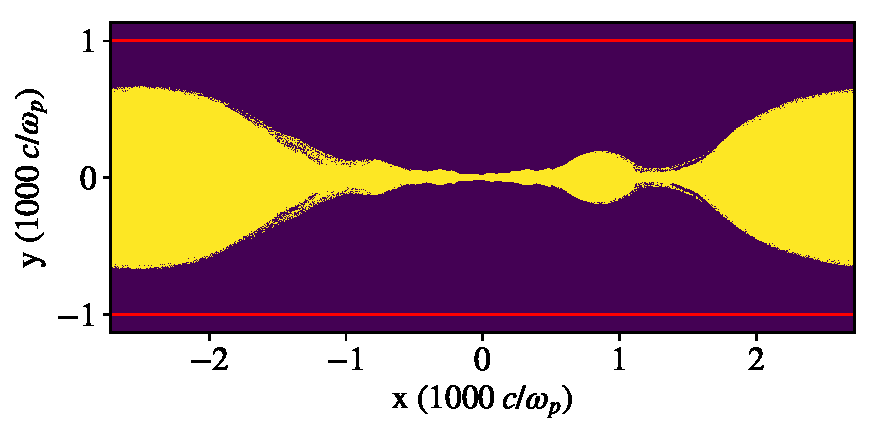
\includegraphics[width=\linewidth]{regions_test.pdf}
\caption{Reconnection region (yellow) identified based on the mixing criterion described in the text. The snapshot refers to the same simulation shown in Figure \ref{lowbeta_threeplot} ($\sigma=0.3$, $\beta=3\times 10^{-4}$, B1), at the last time shown (bottom panel in Figure \ref{lowbeta_threeplot}).  We see that our mixing criterion properly isolates the reconnected overdense plasma from the cold upstream plasma.  The red lines delimit the region in which the total spectra are calculated, as we will discuss in Figure~\ref{timespec}.}
\label{regions}
\end{figure}


\begin{figure}[htp]
	\centering
%\subfloat[Time evolution of the electron energy spectrum (black to red) in  the simulation shown in Figure 1.  The late-time ion energy spectrum is shown in cyan.  ]
{
	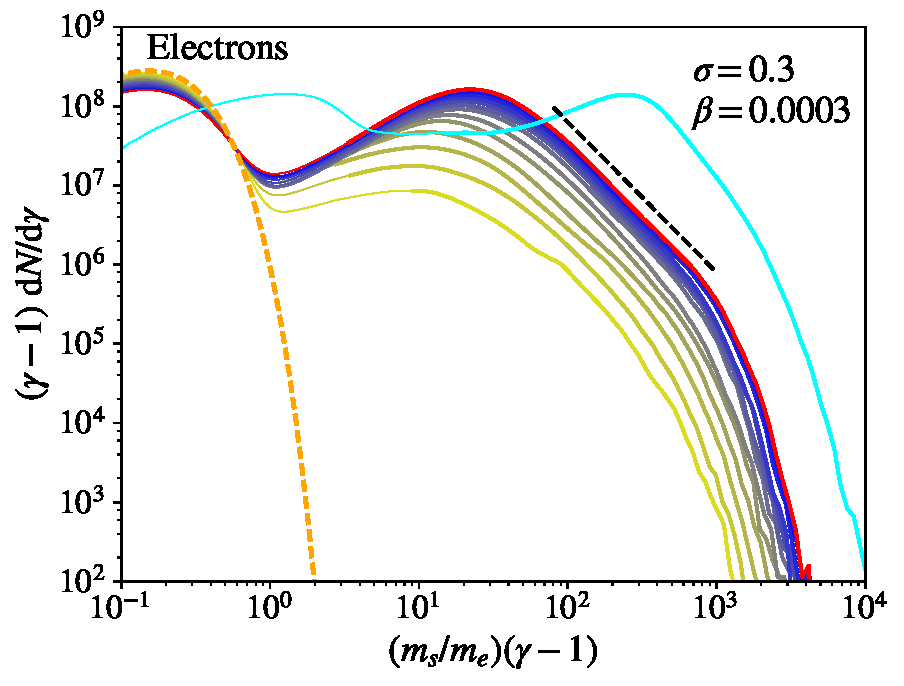
\includegraphics[width=.5\linewidth]{sig_3_delgam00005_timespec.pdf}
}
%\newline
%\subfloat[Time evolution of ion spectra.]
{
	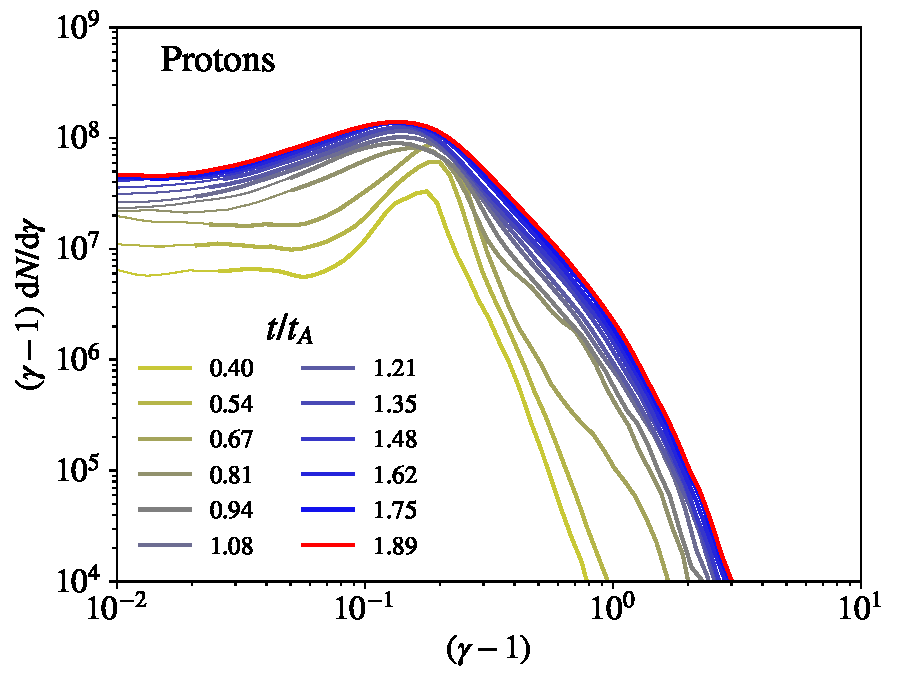
\includegraphics[width=.5\linewidth]{sig_3_delgam00005_timespec_ions.pdf}
}
\caption{Time evolution of the electron (top) and proton (bottom) energy spectra for the simulation shown in Figure \ref{lowbeta_threeplot}, with $\sigma=0.3$ and $\beta=3\times10^{-4}$ (run B1), corresponding to an initial proton thermal spread of $\theta_{i}=5 \times 10^{-5}$. The time sequence (from yellow to blue, with red marking the final time) is indicated in the bottom panel, in units of the Alfv\'enic crossing time $t_A=L_x/v_A$. In each panel, thicker lines indicate the energy range where the spectrum is mostly contributed  by particles in the reconnection region (by more than 75\%). In the top panel, the dashed orange line shows the initial electron Maxwellian for comparison, and the dashed black line represents a power law with slope $p=-d\log{N}/d\log{\gamma}=2.9$.
In the top panel, the proton spectrum at the final time (i.e., red curve in the bottom panel) is overplotted in cyan for comparison, with the horizontal axis rescaled by $m_i/m_e$. Since $m_s=m_e$ for electrons and $m_s=m_i$ for protons, the horizontal axis in the top panel represents the kinetic energy of each species, in units of the electron rest mass.}
\label{timespec}
\end{figure}

\subsection{Time Evolution of the Energy Spectra}
Having seen how the density evolves with time, and where and when various structures such as plasmoids and X-points form, we now examine the time evolution of the electron and proton energy spectra from the same simulation shown in Figure \ref{lowbeta_threeplot}.  We present the time evolution of the electron and proton spectra in the top and bottom panels of Figure \ref{timespec}, respectively. For both species, our spectra only include the particles that start in the ambient plasma (i.e., we exclude the contribution of the hot population that we set up in the current layer, whose properties depend on the initialization of the Harris sheet).  At each time, the spectrum includes all the particles in a fixed region, whose thickness is $\approx 0.2 L_{x}$ on each side of the current  sheet (bounded by the red lines in Figure \ref{regions}). On each curve, a thicker line with the same color marks the energy range where the fractional contribution of the reconnection region (i.e., the yellow region in Figure \ref{regions}) to the overall spectrum is greater than 75\%. So, the sequence of thick lines illustrates the time evolution of the spectrum in the reconnection region (which, from now on, we call ``post-reconnection spectrum'').

In the top panel,  we present the evolution of the electron spectrum, that shows two components. The bump peaking at $\gamma-1 \approx 0.2$ is populated by the cold upstream electrons, and in fact this component is well fit by a Maxwellian distribution with the  temperature that we employ to initialize ambient electrons (dashed orange line). The high-energy component, that peaks at $\gamma \approx 20$, is populated by particles that have been processed by reconnection (in fact, it is plotted with thicker lines, indicating that it is dominated by particles belonging to the reconnection region). The high-energy component is consistent with a single non-thermal population having a power-law slope of $p=-d\log{N}/d\log{\gamma}=2.9$ (as indicated by the dashed black line), that extends from the peak at $\gamma \approx 20$ up to $\gamma\approx1000$, where it cuts off exponentially. The power law starts right at the peak of the high-energy component, a common feature of magnetic reconnection (\citealt{sironi2014}; \citealt{melzani2014b, melzani2014}; \citealt{cerutti2012, cerutti2014, cerutti2017}; \citealt{guo2015}; \citealt{liguo2015};  \citealt{werner2018}). The power-law index is established early on in the evolution of the electron energy distribution, and it does not appreciably change from $t=0.67\,t_{A}$ up to $t=1.89\,t_{A}$. The high-energy cutoff of the electron power law  steadily increases as larger plasmoids form and merge with each other or with the boundary island \citep{sironi2016}. 

In the bottom panel of Figure~\ref{timespec}, we show the time evolution of the proton energy spectrum.  The proton spectrum in the reconnection region resembles a power law at late times, similarly to the electron spectrum. In the top panel, the proton spectrum at the final time ($t=1.89\,t_{A}$) is shown with a cyan line, with the horizontal axis scaled by $m_i/m_e$ in order to compare with the electron spectrum (so, the horizontal axis indicates the kinetic energy of both species, in units of the electron rest mass energy). By comparing the thick cyan line (for protons) with the thick red line (for electrons), we see that the proton mean energy in the reconnection region  is about an order of magnitude larger than the electron mean energy (see \citealt{rowan2017} and \citealt{werner2018} for a discussion of electron and proton heating in trans-relativistic reconnection). We also find that the proton spectrum in the reconnection region has a steeper slope than the electron spectrum, and it spans a smaller range of energies.

The most dramatic difference between electron and proton spectra, though, is in their temporal evolution. At early times, the proton spectrum in the reconnection region (thick lines in the bottom panel) is nearly monochromatic, with a pronounced peak at $\gamma-1 \approx  0.15 \approx  \sigma/2$, as expected from the characteristic kinetic energy of reconnection outflows (moving at $\sim v_A\sim c \,\sqrt{\sigma}$). Starting at $t\approx0.8\,t_A$, the spectrum develops a power-law-like tail. This transition occurs around the time when the two reconnection fronts interact across the periodic boundaries (at a time in between panels (b) and (c) of Figure \ref{lowbeta_threeplot}), forming the large boundary island. This suggests that the interface between the reconnection outflows and the boundary island might be a promising source of non-thermal proton acceleration, as we further discuss in Section \ref{mechanism}. We remark that the development of a non-thermal proton distribution is not a peculiar consequence of our choice of triggering reconnection at the center of our domain. We observe the same evolution of the proton spectrum in untriggered runs, where the tearing mode is allowed to grow spontaneously.

In summary, protons develop a non-thermal tail only after $t\approx0.8\,t_A$, when the two reconnection fronts interact across the periodic boundaries. In contrast, electrons display a non-thermal component since early times. Although we only show here one particular choice of $\sigma$ and $\beta$, this trend holds across all of our low-$\beta$ simulations (the cases with $\beta$ approaching $\beta_{\rm max}$ are an exception, as we discuss below). These differences between the temporal evolution of electron and proton spectra point towards different acceleration mechanisms for the two species, as we discuss further in Section \ref{mechanism}. In particular, we will show that in low-$\beta$ cases, electrons are significantly accelerated at their first interaction with the layer by the non-ideal electric field at X-points. The early evidence for non-thermal electrons then comes from the fact that X-points appear since the earliest stages of evolution of the layer (see Figure \ref{lowbeta_threeplot}).

\begin{figure}[!h]
	\centering
	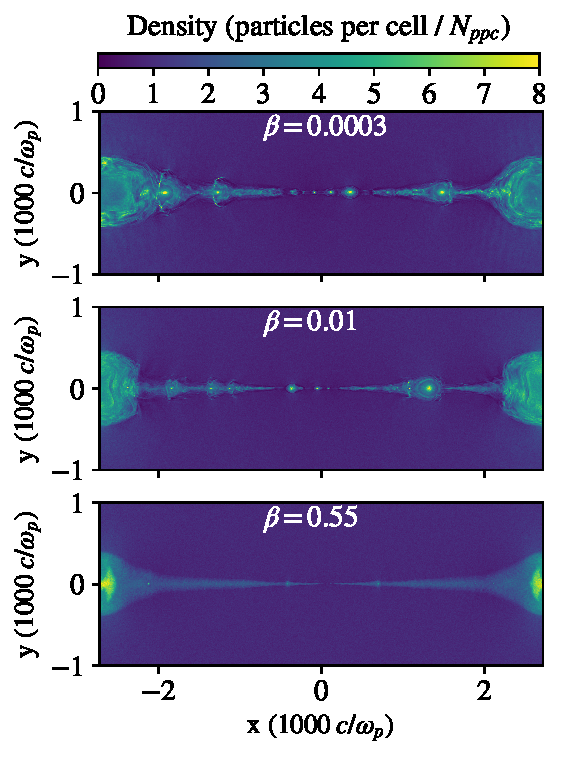
\includegraphics[width =0.5\textwidth]{sig_3_threeplot.pdf}
	\caption{2D density structure  at $t\approx t_{A}$ for a suite of simulations with fixed $\sigma=0.3$ and varying $\beta$: $\beta=0.0003$ (top), $\beta=0.01$ (middle), and $\beta=0.55$ (bottom), corresponding to simulations B1, B5, and B8.  In the lowest-$\beta$ case (top), the reconnection layer is fragmented into numerous plasmoids separated by secondary X-points, whereas the highest-$\beta$ case (bottom) shows a smoother density profile along the reconnection outflows.}
    \label{sig_3_twoplot}
\end{figure}

\begin{figure}[!h]
	\centering
	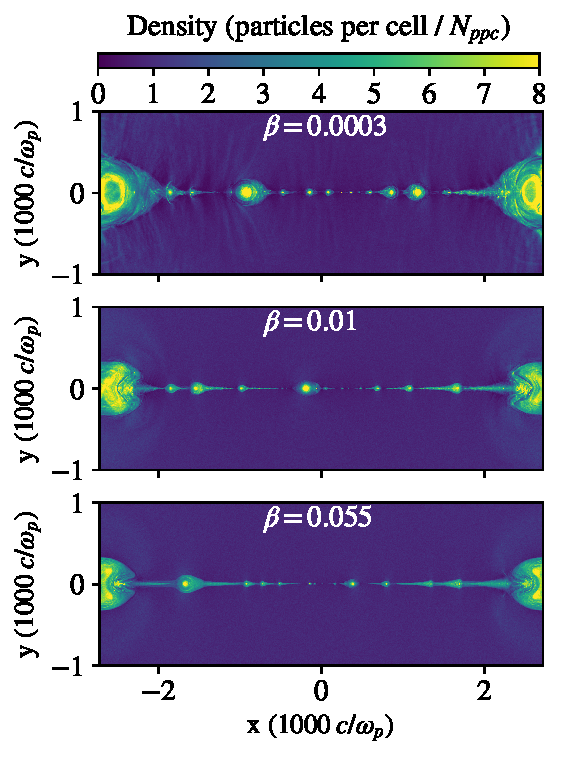
\includegraphics[width =0.5\textwidth]{sig3_threeplot.pdf}
	\caption{2D density structure  at $t\approx t_{A}$ for a suite of simulations with fixed $\sigma=3$ and varying $\beta$: $\beta=0.0003$ (top), $\beta=0.01$ (middle), and $\beta=0.055$ (bottom), corresponding to simulations D1, D4, and D6.  Secondary plasmoids form for all values of $\beta$, with larger plasmoids appearing in the lowest-$\beta$ simulation.}
    \label{sig3_twoplot}
\end{figure}


%%%%%%%%%%%%
\section{The Role of $\beta$ in the Dynamics of the Reconnection Layer}\label{role_of_beta}
In this Section, we illustrate how the dynamics in the reconnection layer depends on plasma beta and magnetization. At first, we study the role of $\beta$ in the  development of 2D structures  in the reconnection region (e.g., secondary plasmoids and X-points), and then we investigate the dependence on $\sigma$ and $\beta$ of the inflow rate (or equivalently, of the rate of magnetic field dissipation). In the next Section, we will study the dependence on $\sigma$ and $\beta$ of the particle energy spectrum.

We show in Figure \ref{sig_3_twoplot} the 2D density structure of three simulations with fixed $\sigma=0.3$ and varying $\beta$: $\beta=0.0003$ (top), $\beta=0.01$ (middle), and $\beta=0.55$ (bottom).  In Figure \ref{sig3_twoplot} we show snapshots from three simulations with $\sigma=3$ (so, one order of magnitude higher than in Figure \ref{sig_3_twoplot}) and different $\beta$: $\beta=0.0003$ (top), $\beta=0.01$ (middle), and $\beta=0.055$ (bottom). For both figures, the snapshots are taken at $t\approx t_{A}$, after the reconnection fronts have reached the boundaries of the box.

In the low-$\sigma$ case (Figure \ref{sig_3_twoplot}, for $\sigma=0.3$), we see a clear difference in the structure of the current sheet between low- and high-$\beta$ simulations (see also \citealt{rowan2017}). At low $\beta$ (top panel), the current layer is pinched by the secondary tearing mode at multiple locations along the sheet, resulting in numerous secondary X-points and plasmoids. In contrast, the highest-$\beta$ case (bottom panel), which is close to $\beta_{\rm max}\approx 1/4\sigma\simeq 0.8$, displays a smooth density profile in the reconnection outflows, with only marginal evidence for two secondary plasmoids. No prominent X-points are detected at high $\beta$ (bottom panel), with the exception of the primary X-point located at the center of the layer, resulting from our initial perturbation of the current sheet.

In the high-$\sigma$ simulations (Figure~\ref{sig3_twoplot}, for $\sigma=3$), the dependence on $\beta$ is less pronounced.  We do, however, see that the lowest-$\beta$ case (top panel) has larger plasmoids and that its current layer is broken up into distinct high-density plasmoids, separated by low-density regions.  In comparison, the highest-$\beta$ simulation in the bottom panel (with $\beta$ approaching $\beta_{\rm max}\approx 1/4\sigma\simeq 0.08$) still presents several secondary plasmoids, but the density profile in between neighboring plasmoids is smoother than at lower $\beta$. In other words, the density contrast between secondary plasmoids and X-points seems to get reduced with increasing $\beta$.

In summary, the fragmentation of the current sheet into secondary plasmoids separated by secondary X-points becomes more and more pronounced at lower $\beta$ (for fixed $\sigma$) and at higher $\sigma$ (for fixed $\beta$; compare the top and middle panels between Figure \ref{sig_3_twoplot}  and Figure~\ref{sig3_twoplot}; see also \citealt{sironi2016}, for the same conclusion in the ultra-relativistic regime $\sigma\gg1$).  It is likely that these structural differences in the appearance of the reconnection layer play a key role in whether efficient particle acceleration occurs, as we will discuss in Section \ref{mechanism}.


\subsection{Reconnection Rate}
In the whole range of $\sigma$ and $\beta$ investigated in this work, we calculate the mean inflow rate, which corresponds to the rate of magnetic field dissipation (i.e., to the so-called ``reconnection rate''). At each time, we compute the spatial average of the $y-$component of the flow velocity in a region close to the center of the domain, covering the range  $|y| \lesssim 400\; c/\omega_{p}$ and $|x| \lesssim 1000\; c/\omega_{p}$. This area is sufficiently large that it allows to obtain a proper estimate of the steady-state inflow rate, and it is chosen to exclude the boundary island, that artificially inhibits the plasma inflow rate in its vicinity. 

In Figure \ref{sigpoint3_inflow_rates}, we show the temporal evolution of the inflow rate for four representative simulations, having a fixed $\sigma=0.3$ and ranging in $\beta$ over three orders of magnitude. The inflow speed is measured in units of the upstream Alfv\'{e}n velocity $v_A$. At early times ($\omega_{p}t\lesssim 5000$), the inflow rate steadily increases, as the reconnection fronts move away from the center of the domain, and the region of inflowing plasma  extends further and further in both the $x$ and $y$ directions. 
After the reconnection rate reaches its peak, it settles around a constant value (with only a slight decrease at later times). Eventually, the boundary island would grow so large to inhibit the inflow of particles and magnetic flux, and the reconnection rate would artificially drop to zero. Figure \ref{sigpoint3_inflow_rates} suggests that, for the timespan covered by our simulations, the computational domain is sufficiently large to properly capture the steady state of reconnection, without artificial effects from the periodic boundaries.

At low $\beta$  (most notably for $\beta=10^{-4}$ and $\beta=10^{-3}$, cyan and green lines), the inflow rate displays significant fluctuations. After the peak, the reconnection rate drops. This is due to the fact that 
the first secondary plasmoids tend to form around the center of the box, and their pressure slightly inhibits the inflow of surrounding upstream plasma. Once the plasmoids get advected by the field tension towards the boundary island, the upstream plasma can freely flow into the layer, which explains the second peak in the reconnection rate (at $\omega_{p}t\sim 9500$ for $\beta=10^{-4}$ and at $\omega_{p}t\sim 13000$ for $\beta=10^{-3}$). These oscillations in the temporal profile of the inflow rate are observed for all our low-$\beta$ cases.

\begin{figure}[!h]
	\centering
{
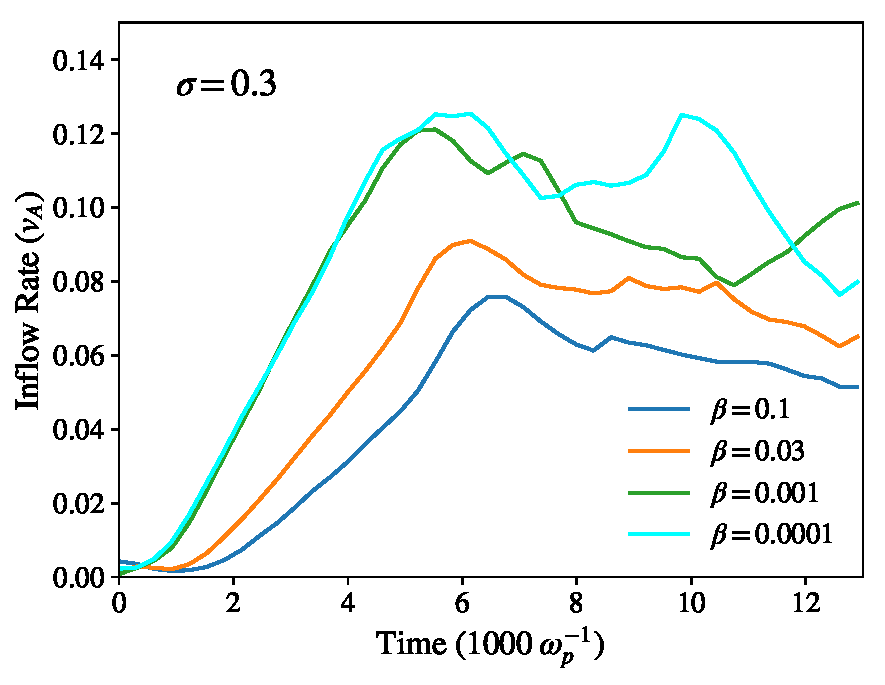
\includegraphics[width=\linewidth]{sigpoint3_inflow_rates.pdf}
\caption{\label{sigpoint3_inflow_rates}Time evolution of the inflow rate, in units of the upstream Alfv\'en speed, for four different simulations at fixed $\sigma=0.3$ and varying $\beta$ (simulations B0, B2, B6, and B7, in order of increasing $\beta$).  The inflow speed tends to decrease at higher $\beta$.}
}
\end{figure}

From  Figure \ref{sigpoint3_inflow_rates}, it is clear that the inflow rate is nearly independent of $\beta$ in the low-$\beta$ regime, but it tends to decrease at higher $\beta$. This is further confirmed by Figure~\ref{inflow_rates_over_Va}. There, we present, as a function of $\sigma$ and $\beta$, the mean reconnection rate, averaged from the peak time through a timespan of $3000 \; \omega_{p}^{-1}$ ($\sim 0.3 \,t_{A}$), when the reconnection process is  steadily active. The error bars in Figure \ref{inflow_rates_over_Va} indicate the standard deviation, which is larger at lower $\beta$, where the copious formation of secondary plasmoids causes pronounced oscillations in the inflow rates, as we have discussed above.

From Figure \ref{inflow_rates_over_Va}, we see that the inflow rate for $\beta\gtrsim 10^{-2}$ is nearly independent of $\sigma$, but it gets lower and lower for increasing $\beta$ (as already observed in MHD simulations by \citealt{ni2012}, and in PIC simulations by \citealt{rowan2017}). For $\beta\lesssim 10^{-2}$, the inflow rate is nearly $\beta$-independent (with the exception of $\sigma=3$), and tends to increase with $\sigma$ when approaching the relativistic regime $\sigma\gtrsim 1$ (see  \citealt{sironi2016} for the dependence of the inflow rate on magnetization in the ultra-relativistic regime $\sigma\gg1$). The low-$\beta$ limit at $\sigma\lesssim1$ is consistent with a fixed value of the reconnection rate, of order $\sim 0.1\,v_{A}$. 
As we further discuss in the next two Sections, the dependence of the inflow velocity on $\beta$ and $\sigma$ will be mirrored by the magnitude of the electric field in the reconnection region, which in turn impacts the rate of particle acceleration.

%In addition to the inflow rate, we have also analyzed the dependence on $\beta$ and $\sigma$ of the outflow speed. While the inflow rates are highly sensitive to $\beta$, the speed of outflowing plasma is largely independent of the plasma-$\beta$, almost always reaching of order the Alfv\'en velocity (see \citealt{rowan2017} for a detailed analysis of the $\beta$-dependence of the outflow velocity).

%\begin{figure}[b]
%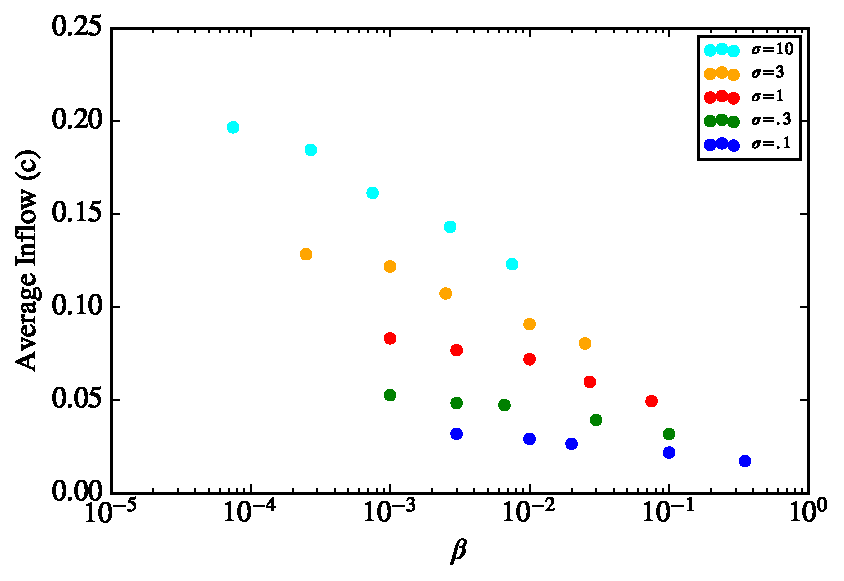
\includegraphics[width =0.5\textwidth]{inflow_rates.pdf}
%	\caption{Inflow rates across $\sigma$, $\beta$, in units of the speed of light}
%    \label{inflow_rates}
%\end{figure}


\begin{figure}[t]
	\centering
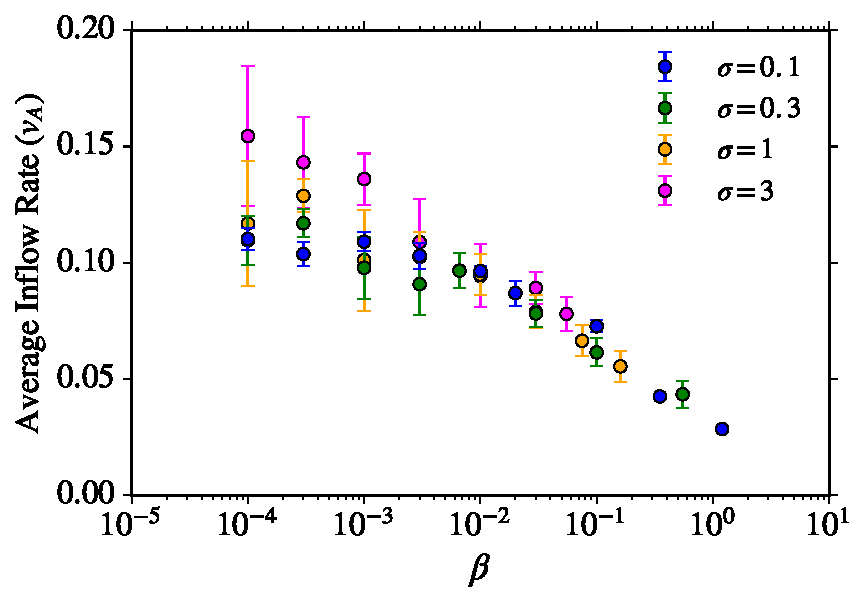
\includegraphics[width =\textwidth]{inflow_rates_over_va.pdf}
	\caption{Temporal averages of the inflow rate as a function of $\sigma$ and $\beta$, in units of the upstream Alfv\'en velocity.  The error bars indicate the standard deviation, which is larger at low $\beta$ for the copious formation of secondary plasmoids.}
    \label{inflow_rates_over_Va}
\end{figure}


\section{Dependence on  $\beta$ and $\sigma$ of the Electron Energy Spectra}\label{energy_spectra}
In this Section, we investigate the role of $\sigma$ and $\beta$ on the physics of non-thermal particle acceleration, with focus on electron acceleration. We first describe how we characterize the non-thermal electron energy spectrum in the reconnection region, finding that it can be generally modeled as a power law. We quantify how the slope of the power law and the electron acceleration efficiency depend on $\beta$ and $\sigma$. We also discuss an additional high-energy component that appears for $\beta$ approaching $\beta_{\rm max}$ in both electron and proton spectra.

%We now turn to the electron energy spectra and quantify the non-thermal component that emerges as a result of reconnection as a function of the plasma parameters.
 
\subsection{Characterizing the Electron Energy Spectra}\label{chara}
As an illustrative example of how we characterize the properties of electron spectra, we show in Figure~\ref{spec_fit_ex} the electron energy distribution for a simulation with $\sigma=0.3$ and $\beta=0.003$. The solid blue line depicts the electron spectrum measured in a slab with $|y|\lesssim 1000\,c/\omega_{p}$, as delimited by the red lines in  Figure \ref{regions}. The portion of the blue curve plotted with a thicker blue line in Figure~\ref{spec_fit_ex} indicates the energy range where the reconnection region (yellow area in  Figure \ref{regions}) contributes more than 75\%. The dashed orange line shows the Maxwellian distribution initialized in the inflow region, demonstrating that the low-energy bump in the electron spectrum is populated by particles that have yet to experience the reconnection process (and so, they should not be accounted for, when drawing conclusions on the post-reconnection particle spectrum). The high-energy component (thick blue line) is a genuine by-product of the reconnection physics. It can be modeled as a power law (compare with the dashed red line, that has a slope of $p=2.9$).

In addition to the power-law slope, we quantify the efficiency of reconnection in producing non-thermal particles, by employing the following strategy. We isolate the spectrum of the reconnection region (thick blue line), and fit its peak with a relativistic Maxwellian $f_{\rm MB} (\gamma,\theta)$ (dashed blue line in Figure~\ref{spec_fit_ex}, having a thermal spread $\theta=kT/m_e c^2\approx8$). If $\gamma_{\rm pk}$ is the peak of the electron spectrum in the reconnection region, the spectrum at $\gamma\geq \gamma_{\rm pk}$ will exceed the Maxwellian distribution (i.e., in Figure~\ref{spec_fit_ex} the thick solid blue line lies above the dashed blue line).
We then quantify 
the electron acceleration efficiency by integrating at $\gamma\geq \gamma_{\rm pk}$ the excess of the electron spectrum with respect to the best-fitting Maxwellian, normalized to the overall energy content of the spectrum. Thus, the non-thermal acceleration efficiency $\epsilon$ is defined as
\begin{equation}
\epsilon= \frac{\int_{\gamma_{\rm{pk}}}^{\infty}(\gamma-1)[ \frac{dN}{d\gamma} -f_{\rm MB}(\gamma,\theta)]d\gamma}{\int_{\gamma_{\rm pk}}^{\infty}(\gamma-1) \frac{dN}{d\gamma}d\gamma}~,
\label{efficiency_eqn}
\end{equation}
where $\theta$ is the best-fitting thermal spread. 

In Section \ref{sec:5.4}, we will employ this strategy to characterize how the non-thermal acceleration efficiency and the electron power-law slope depend on plasma beta and magnetization. We will take the electron spectrum at $t\approx 2\,t_{A}$, when the spectral shape has saturated. At this time, most of the high-energy electrons reside in the boundary island, which acts as a reservoir of particles. 

We conclude this Subsection with two remarks. First, as we discuss in Section \ref{sec:5.2}, the electron spectrum tends to soften with increasing $\beta$, so its deviations from a Maxwellian  become smaller and smaller. It follows that our determination of the electron power-law slope and non-thermal efficiency become less accurate for higher $\beta$. 

Second, as we describe in Section \ref{betamax}, a peculiarity of the extreme cases with $\beta\sim \beta_{\rm max}$ is the presence of a separate high-energy spectral component, containing a few percent of particles (the simulations where this happens are marked with an asterisk in Table 1). As we discuss below, the particles belonging to this additional component experience a different energization process than the bulk of electrons accelerated by reconnection. For this reason, we neglect this additional component when characterizing the non-thermal acceleration efficiency. In practice, for the small set of simulations with $\beta\sim \beta_{\rm max}$, we identfy the Lorentz factor where the additional component starts, and we take this as an upper limit in Equation \ref{efficiency_eqn}, rather than integrating up to infinity. 
  

\begin{figure}[!t]
	\centering
	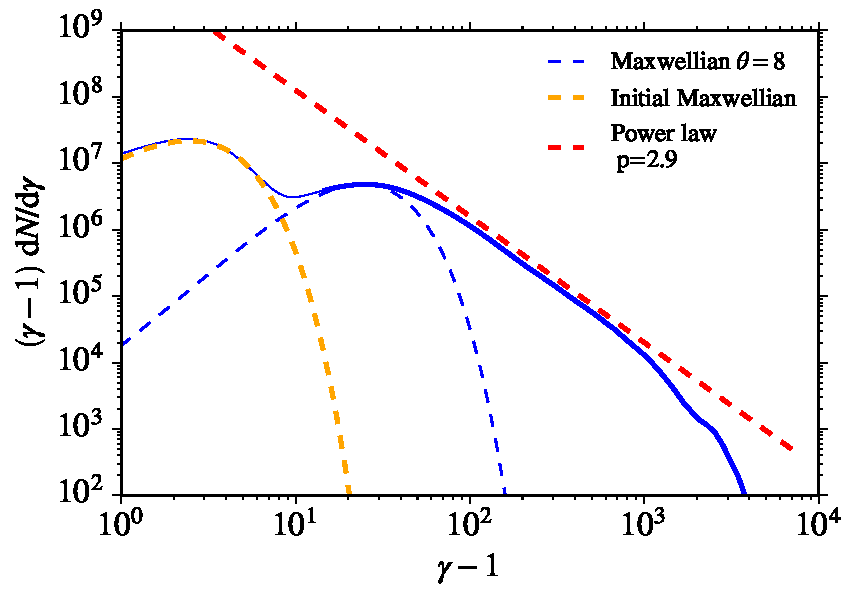
\includegraphics[width =\textwidth]{single_powerlaw_fit.pdf}
	\caption{Electron spectrum for a simulation with $\sigma=0.3$ and $\beta=0.003$ (simulation B3) taken at $t=2\,t_{A}$.  The solid blue line shows the overall spectrum in the slab delimited by the red lines in Figure~\ref{regions}, and the thick blue line marks the energy range where the spectrum is mostly contributed by the reconnection region (yellow area in Figure~\ref{regions}).  The dashed blue line shows the Maxwellian fit to the peak of the spectrum in the reconnection region, the red dashed line shows the best-fitting power law, and the orange dashed line depicts the  Maxwellian distribution initialized in the inflow region.}
\label{spec_fit_ex}
\end{figure}


\begin{figure}[!b]
	\centering
	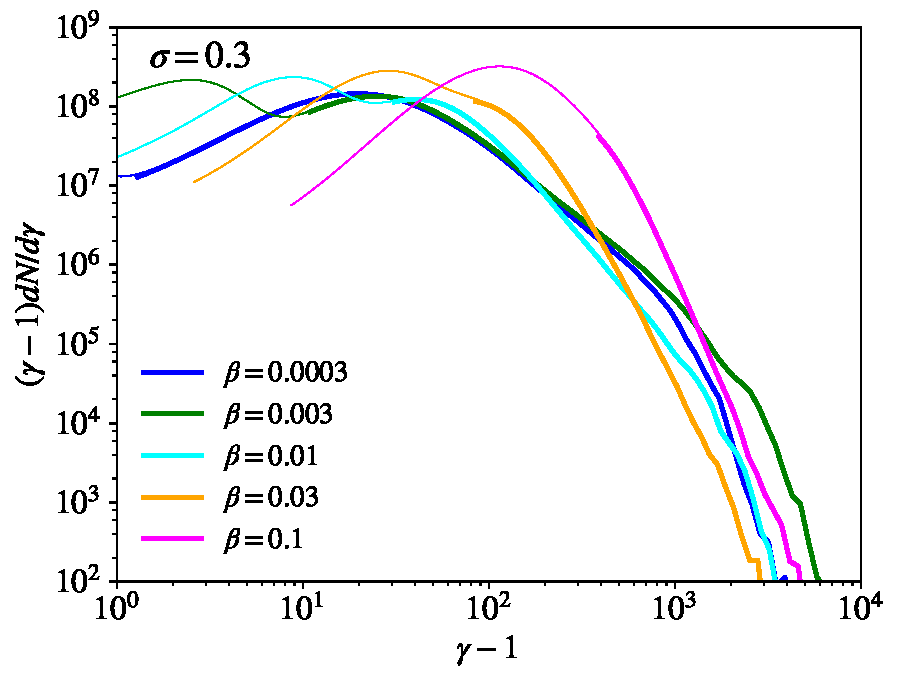
\includegraphics[width =\textwidth]{sig_3_betas_withcold.pdf}
	\caption{Electron spectra for fixed $\sigma=0.3$ and varying $\beta$, as indicated in the legend (simulations B1, B3, B5, B6, and B7), calculated at $t\approx 2\,t_{A}$.  At low $\beta$, the spectral shape converges (e.g., the blue and green curves have the same spectral slope), but as $\beta$ increases, the power law steepens significantly. Thicker lines indicate post-reconnection spectra.}
    \label{sig_3_betas_lecs}
\end{figure}

\subsection{Dependence on $\beta$  and $\sigma$ of Electron Energy Spectra}\label{sec:5.2}
In this Section, we present a few representative electron energy spectra, to illustrate the dependence on $\beta$  and $\sigma$. All  the spectra are measured at $t=2\, t_{A}$. As usual, thicker lines indicate the spectral range dominated by particles residing in the reconnection region (i.e., they display the post-reconnection spectra). 

In Figure~\ref{sig_3_betas_lecs}, we show five electron spectra from simulations with fixed $\sigma=0.3$ and a wide range of $\beta$ (see the legend). 
At low beta ($\beta\lesssim 3\times 10^{-3}$), the post-reconnection spectra (blue and green thick lines) peak at $\gamma\sim 20$, regardless of $\beta$. This is consistent with the results in \citet{rowan2017}, where it was shown that, at sufficiently low $\beta$, the reconnection process converts a fixed amount of magnetic energy into electron energy, regardless of the initial $\beta$
(so, regardless of the location of the peak in the thin lines). In addition, Figure~\ref{sig_3_betas_lecs} shows that  the shape of the post-reconnection spectrum is nearly the same for all values of $\beta\lesssim 3\times10^{-3}$. Both the power-law slope and the high-energy cutoff are insensitive to the plasma beta, in the range $\beta\lesssim 3\times 10^{-3}$. The small degree of variation in the slope and high-energy cutoff between the cases with $\beta=3\times10^{-3}$ (green) and $\beta=3\times10^{-4}$ (blue) is due to the stochastic nature of the plasmoid chain. In fact, in the $\beta=3\times10^{-3}$ simulation (green line in Figure~\ref{sig_3_betas_lecs}), a sequence of consecutive mergers leads to the formation of an unusually large secondary plasmoid. Each merger is accompanied by efficient electron acceleration (see Section \ref{mechanism}), and the peculiar merger history of the $\beta=3\times10^{-3}$ case results in the high-energy slope being slightly harder and extending to higher energies than in other simulations with comparable $\beta$ (and than in the case $\beta=3\times10^{-4}$ indicated by the blue line).

At higher beta ($\beta\gtrsim 10^{-2}$), the separation between the thermal peak of inflowing particles (thin lines) and the post-reconnection component (thick lines) shrinks, since the energy content in magnetic fields available for dissipation becomes a smaller and smaller fraction of the plasma thermal energy (compare the cyan, yellow and pink lines). In these high-$\beta$ cases, the spectrum of the plasma that has undergone reconnection can only be identified thanks to our mixing criterion, which is based on the spatial distinction between the upstream flow and the post-reconnection region (rather than on a distinction in energy space, which is impossible at high $\beta$, as Figure~\ref{sig_3_betas_lecs} shows). With increasing $\beta\gtrsim 10^{-2}$, we find that the power-law slope steadily steepens (compare green, cyan and yellow curves), and the overall spectrum  eventually resembles a single Maxwellian distribution (see the pink line). This trend holds for all the magnetizations we have investigated, as we further discuss in Section \ref{sec:5.4}.

In Figures~\ref{beta0003_spec} and \ref{beta01_spec}, we explore how the electron spectra change when varying $\sigma$, at fixed $\beta$. As $\sigma$ increases, the amount of magnetic energy available for dissipation increases, which explains the shift to higher and higher energies in the peaks of post-reconnection spectra. 
More interestingly, for $\beta=3\times10^{-4}$ (Figure~\ref{beta0003_spec}), we see that the post-reconnection spectrum becomes significantly harder with increasing $\sigma$.  The same is observed for $\beta=0.01$ (Figure~\ref{beta01_spec}), although the trend is not as prominent.

This trend --- of harder spectral slopes for higher $\sigma$ --- has been already discussed by \citet{werner2018}. In fact, the four simulations  in Figure~\ref{beta01_spec} have the same physical parameters as in \citet{werner2018}, where the dependence on $\sigma$ was investigated for the specific case of $\beta=0.01$.
In \citet{werner2018}, the electron power-law slopes for $\sigma=0.1, \; 0.3, \; 1,$ and $ 3$ were measured to be 4.0, 3.3, 2.8, and 2.4, respectively.  For these same values of $\sigma$ and $\beta$, we measure power-law indices of 4.3, 3.8, 3.6, and 3.2, i.e., we find that our spectra are systematically softer than in \citet{werner2018}. We attribute this discrepancy to the combination of two effects. First, our simulation domain for $\beta=0.01$ is about five times larger than in \citet{werner2018} (in Table 1, compare with their choice of $L_x=120\,r_{e,\rm hot}$). As we  discuss in Appendix \ref{boxsize}, larger domains systematically lead to steeper electron spectra. Second, as we describe in Appendix \ref{untriggered}, we find appreciable differences in the hardness of the electron spectrum between our setup, where reconnection is triggered in response to a large-scale perturbation, and the untriggered case, where the system evolves from particle noise. In particular, the untriggered setup generally leads to harder electron spectra. We have verified that we  recover the power-law slopes quoted by  \citet{werner2018} in the case of untriggered simulations with the same box size that they employ.


\begin{figure}[!h]
	\centering
	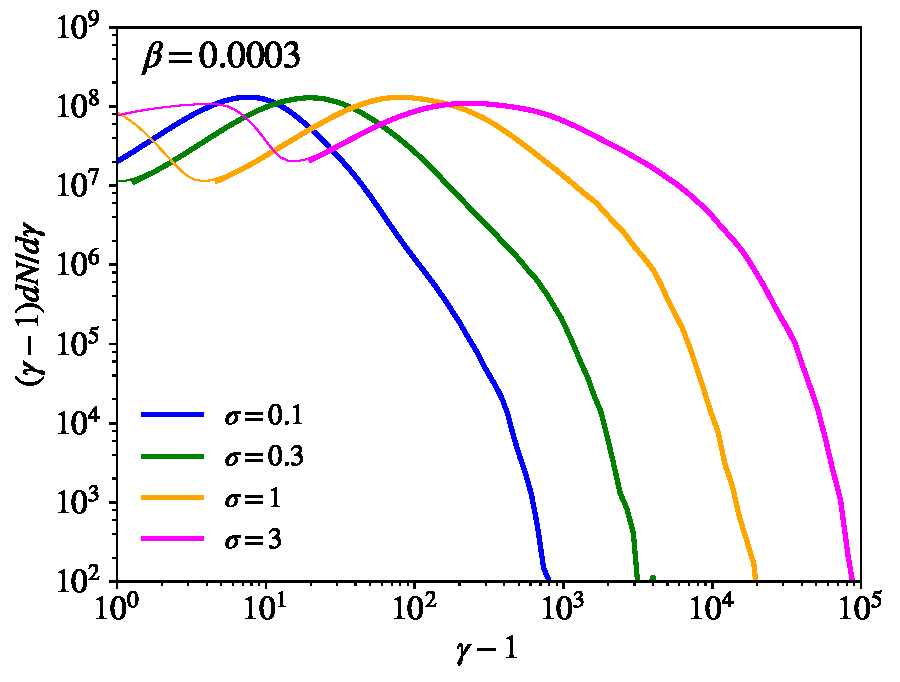
\includegraphics[width =\textwidth]{beta_0003_sigmas_withcold.pdf}
	\caption{Electron spectra for a set of simulations with fixed $\beta=3\times 10^{-4}$ and varying $\sigma$, as indicated in the legend (simulations A1, B1, C1, and D1), measured at $t\approx 2\,t_{A}$.  As $\sigma$ increases, the spectra broaden and the slope hardens.}
    \label{beta0003_spec}
\end{figure}

\begin{figure}[!h]
	\centering
	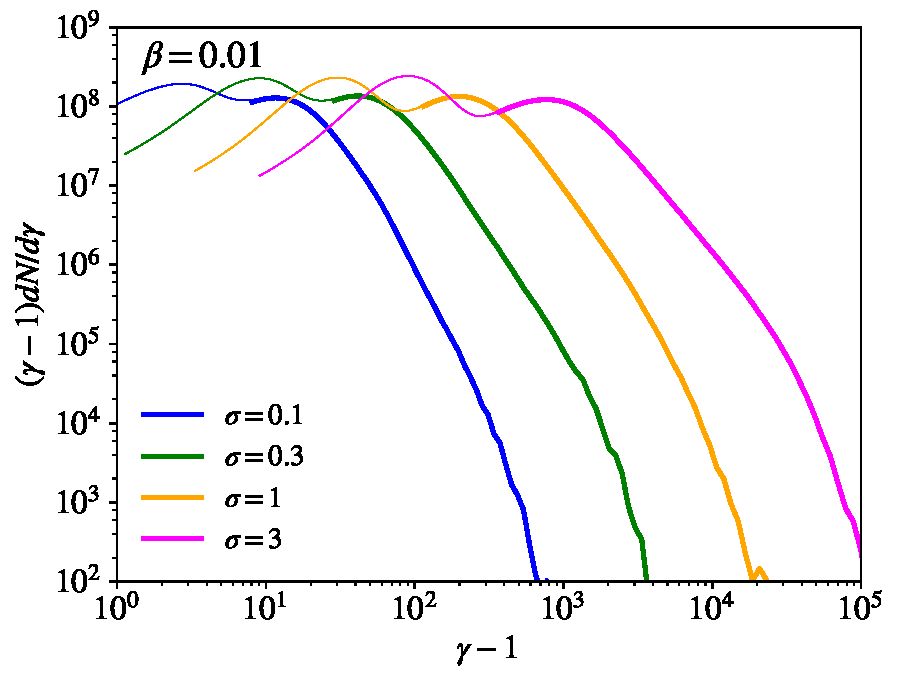
\includegraphics[width =\textwidth]{beta_01_sigmas_withcold.pdf}
	\caption{Electron spectra for a set of simulations with fixed $\beta=0.01$ and varying $\sigma$, as indicated in the legend (simulations A4, B5, C4, and D4), measured at $t\approx 2\,t_{A}$. This choice of $\beta$ is the same as in the work by  \citet{werner2018}.}
    \label{beta01_spec}
\end{figure}

\subsection{The Additional High-Energy Component at $\beta \sim \beta_{\rm max}$}\label{betamax}
A peculiarity of the extreme cases with $\beta\sim \beta_{\rm max}$ (marked with an asterisk in Table 1) is the presence of a separate high-energy spectral component emerging at late times. In Figure \ref{sig1_timespec}, we show  the temporal evolution of the electron spectrum in the simulation  that shows the strongest evidence for this additional component (i.e., the case with $\sigma=1$ and $\beta=0.16$).  

At early times ($t\lesssim t_{A}$), the high-energy part of the spectrum is very steep, barely emerging from the upstream Maxwellian (indicated by the orange dashed line). At later times ($t\gtrsim t_{A}$), an additional component appears at high energies, containing a few percent of electrons. It develops around the time when the boundary island is formed by the interaction of the two reconnection fronts across our periodic boundaries. As we show in Section \ref{mechanism}, the electrons belonging to this additional high-energy component are accelerated by bouncing between the reconnection outflow and the boundary island, in a process reminiscent of the Fermi mechanism. We remark that, as we discuss in Appendix \ref{untriggered}, this additional high-energy component is a generic outcome of high-$\beta$ reconnection. In particular, it is not an artificial by-product of our choice of a triggered reconnection setup, since it also appears in untriggered simulations. 

In Figure \ref{sig1_timespec}, we also show with a cyan line the proton spectrum at the final time (with the horizontal axis rescaled by the mass ratio, to facilitate comparison with the electron spectrum). We find that the proton spectrum displays a similar high-energy component, with just a slightly higher normalization (i.e., a slightly larger injection efficiency into the acceleration process). In other words,  electrons and protons are subject to the same  acceleration mechanism.
In retrospect, this is not surprising: in the limit that $\beta$ approaches $\beta_{\rm max}$, the upstream protons become trans-relativistic ($\theta_{i}=0.2$ for the case we show). Since the upstream electrons are also relativistic, the two species have comparable Larmor radii, and are then expected to be accelerated in a similar fashion.
 
 

\begin{figure}[!h]
\centering
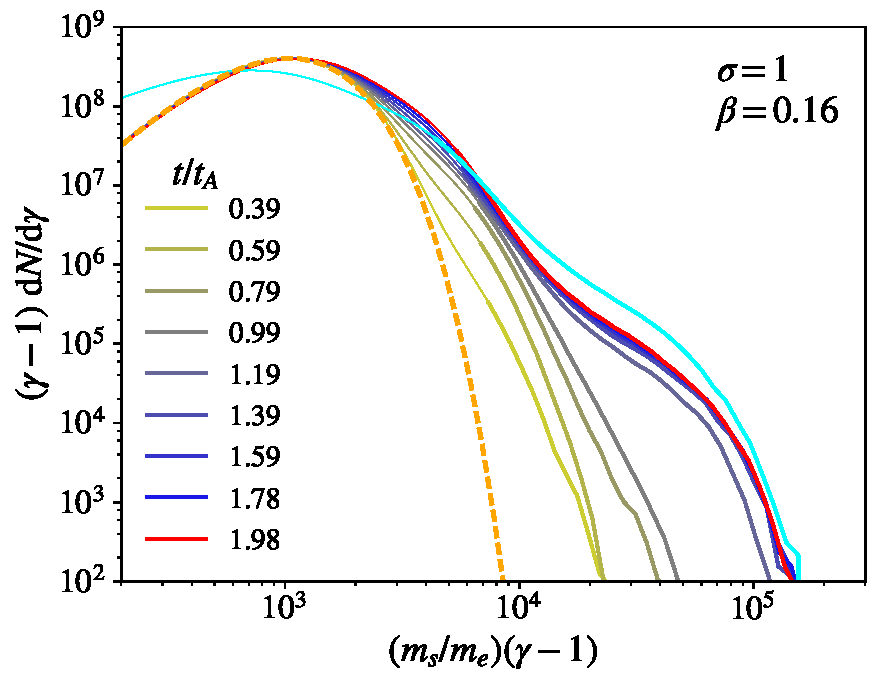
\includegraphics[width =\textwidth]{sig1_delgam_2_timespec.pdf}
\caption{Time evolution of the electron spectrum in the simulation with $\sigma=1$ and $\beta=0.16$ (simulation C7) that shows the strongest evidence for the additional high-energy component seen as $\beta\rightarrow\beta_{\rm max}$. We show the upstream electron Maxwellian with a dashed orange line. The proton spectrum at the final time is shown with the cyan line, with the horizontal axis rescaled by the mass ratio for comparison. Time is in units of the Alfv\'enic crossing time $t_A=L_x/v_A$.}
\label{sig1_timespec}
\end{figure}






%\begin{figure}[!h]
%	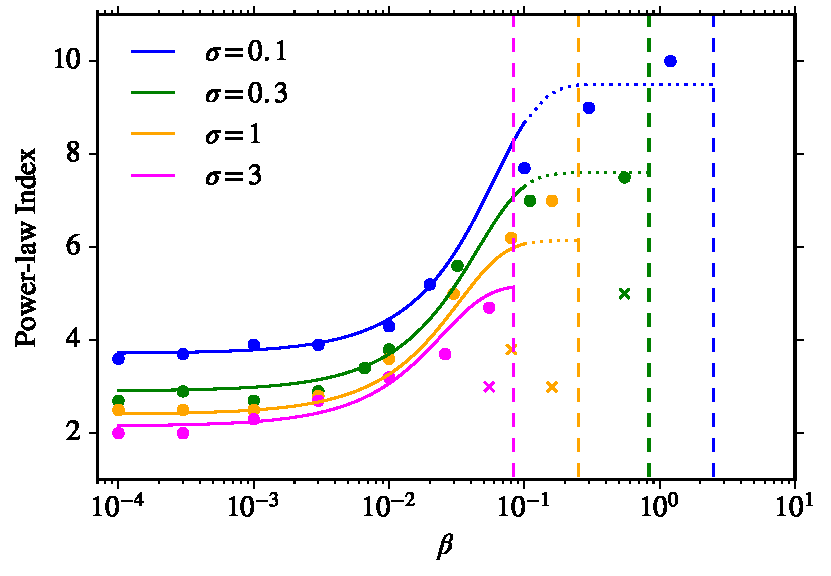
\includegraphics[width =0.5\textwidth]{powerlaw_fit.pdf}
%	\caption{Plasma-$\beta$ vs. power-law index of electron spectra.  The x's show the slopes of the hardened spectra from the secondary shock-type acceleration that occurs at high-$\beta$.}
%    \label{beta_vs_p}
%\end{figure}


%\begin{figure}[!h]
%	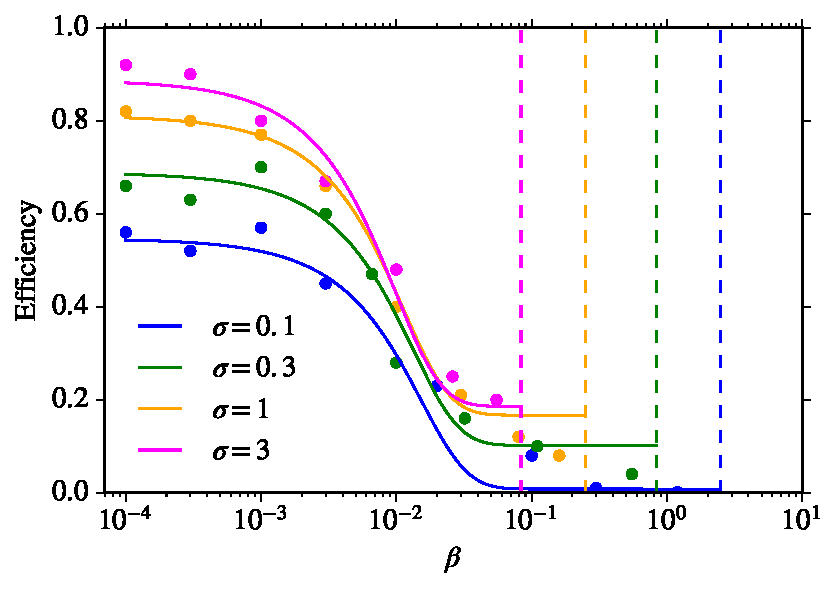
\includegraphics[width =0.5\textwidth]{efficiency_fit.pdf}
%	\caption{Plasma-$\beta$ vs. efficiency of nonthermal acceleration, defined as the ratio of nonthermal energy to total energy.}
%   \label{beta_vs_eff}
%\end{figure}

%\begin{figure}[!h]
%	\includegraphics[width =0.5\textwidth]{sig_3_betas_final_ions.png}
%	\caption{Ion spectra in the reconnection region at $\sigma=0.3$ across numerous values of $\beta$.}
%    \label{sig_3_betas_ions}
%\end{figure}



\subsection{Dependence on $\beta$  and $\sigma$ of the Power-Law Slope and Acceleration Efficiency}\label{sec:5.4}
In this Section, we summarize our results on the dependence of the electron energy spectrum on magnetization and plasma beta. In particular, in Figure \ref{powerlaw_fit} we show how the electron power-law slope depends on $\beta$ and $\sigma$, whereas in Figure  \ref{efficiency_fit} we present the dependence on $\beta$ and $\sigma$ of the efficiency of non-thermal electron acceleration, as defined in Equation \ref{efficiency_eqn}.  

In Figure \ref{powerlaw_fit}, filled circles indicate the slope of the main component of accelerated electrons, while crosses represent the slope of the additional component that emerges for $\beta\approx \beta_{\rm max}$ at late times (in the plot, the values of $\beta_{\rm max}$ for each $\sigma$ are indicated by the vertical dashed lines). When focusing on the filled circles, two trends are evident. First, at fixed $\beta$, the power-law slope is harder for higher $\sigma$ (see also \citealt{werner2018}). Second, at fixed $\sigma$ (i.e., fixed color), the slope is independent of $\beta$ for $\beta \lesssim 3 \times 10^{-3}$, but it increases (so, corresponding to a softer spectrum) at higher $\beta$, eventually resulting in a non-thermal tail that is so steep to be indistinguishable from the high-energy end of a Maxwellian distribution.

\begin{figure}[!h]
\centering
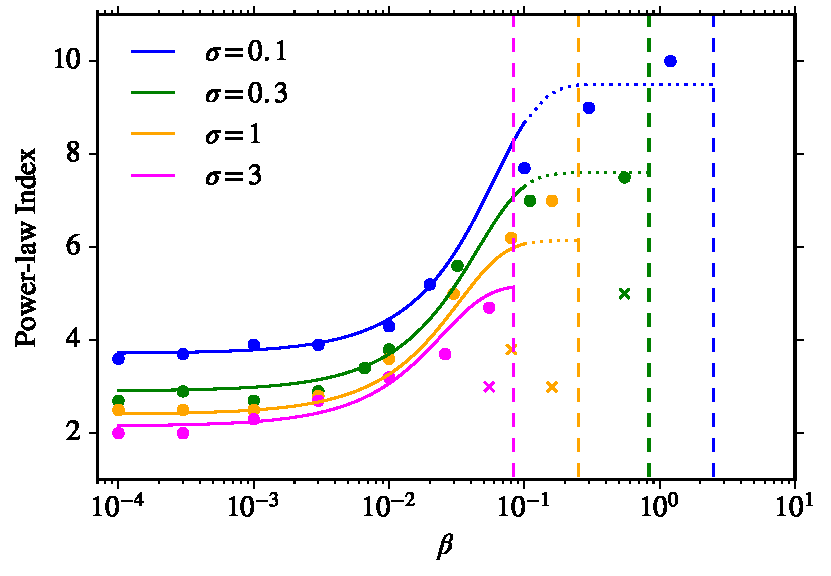
\includegraphics[width =\textwidth]{powerlaw_fit.pdf}
\caption{Electron power-law slope as a function of $\beta$ (horizontal axis) and for different values of $\sigma$ (different colors, as indicated in the legend).  The power-law indices of the main non-thermal component (i.e., the one starting from the thermal peak) are depicted with filled circles, while the power-law indices of the additional high-energy bump that appears for $\beta\sim \beta_{\rm max}$ (i.e., in the simulations marked with an asterisk in Table 1) are indicated with crosses.  The solid lines show our empirical fit in Equation \ref{initial_tanfit}. Beyond $\beta\sim 0.1$, the electron spectra become very steep and so our estimates are less robust (for this reason, our fitting curves for $\beta\gtrsim 0.1$ are plotted as dotted lines).  The values of $\beta_{\rm{max}}$ for each $\sigma$ are indicated with vertical dashed lines.}
\label{powerlaw_fit}
\end{figure}

The combined dependence of the electron slope $p$ on plasma $\beta$ and magnetization $\sigma$ can be empirically fit as 
\begin{equation}
p = A_{p} + B_{p} \tanh{(C_{p}\beta)}~~,
\label{initial_tanfit}
\end{equation}
where
\begin{equation}
\begin{aligned}
A_{p}=1.8 + 0.7/\sqrt{\sigma}~,~B_{p}=3.7\,\sigma^{-0.19}~,~C_{p}=23.4\,\sigma^{0.26}   ~.   
\end{aligned}
\label{powerlaw_fit_params}
\end{equation}
The fits are shown in Figure \ref{powerlaw_fit}  with solid lines, having the same color coding as the filled circles. For $A_p$, we have employed an expression similar to \citet{werner2018}, which properly captures the $\sigma$-dependence of our results in the limit $\beta\ll1$ (in practice, for $\beta\lesssim 3\times 10^{-3}$ we can approximate $p\simeq 1.8 + 0.7/\sqrt{\sigma}$). In particular, at $\beta\ll1$ the electron power-law slope approaches $p\simeq 1.8$ in the ultra-relativistic regime $\sigma\gg1$, whereas $p\rightarrow+\infty$ in the non-relativistic limit $\sigma\ll1$ (so, no appreciable electron acceleration in non-relativistic reconnection).

We remark that our fit is meant to capture the dependence on $\sigma$ and $\beta$ of the main component of the electron spectrum, i.e., we exclude the additional high-energy component found for $\beta\sim\beta_{\rm max}$ (so, we fit the trend in the filled circles, neglecting the crosses). Also, our fit should be employed only up to $\beta\sim 0.1$. At higher $\beta$, the electron spectra are very steep, so the power-law slope is not well constrained (as shown below, the non-thermal acceleration efficiency is negligible for $\beta\gtrsim 0.1$). For this reason, the fits above $\beta\sim0.1$ are indicated with dotted lines,  cautioning that our estimates at high $\beta$ are not very robust. 

%We find that our expression for the power-law index of a cold plasma ($\beta 3\times 10^{-3}$) is in good agreement with that presented in \citet{werner2018} (who had $\beta = 0.01$): we find $p\approx 1.8 + 0.7/\sqrt{\sigma}$, as compared to $p\approx 1.9 + 0.7/\sqrt{\sigma}$ in that study.  Note, however, that this apparent agreement is due to the fact that they use a higher plasma-$\beta$ (which softens the slope), but a much smaller box (which hardens the slope, see Appendix \ref{boxsize}).  These two effects happen to cancel eachother out for their particular choice of $\beta$. 

In addition to the power-law slope, we have also quantified the dependence on $\beta$ and $\sigma$ of the efficiency of non-thermal electron acceleration, as defined in Equation \ref{efficiency_eqn}.\footnote{As discussed in Section \ref{chara}, we remind that our calculation of the non-thermal efficiency excludes the high-energy component emerging for $\beta\sim \beta_{\rm max}$, since it results from a different energization process than the bulk of reconnection-accelerated electrons.} As shown in Figure \ref{efficiency_fit}, the dependence of the efficiency on $\sigma$ and $\beta$ mirrors the trends described above for the power-law slope. At low $\beta$ ($\beta \lesssim 3 \times 10^{-3}$), where the power-law slope is hard, the efficiency saturates at a value that is independent of $\beta$, and that is systematically larger for higher $\sigma$ (see the legend). At $\beta \gtrsim 3 \times 10^{-3}$, the electron spectrum becomes softer and softer with increasing $\beta$, eventually approaching a Maxwellian, so that the non-thermal efficiency drops to zero.

The combined dependence of the electron non-thermal efficiency $\epsilon$ on plasma $\beta$ and magnetization $\sigma$ can be empirically fit as 
\begin{equation}
\epsilon = A_{\epsilon} + B_{\epsilon} \tanh{(C_{\epsilon}\beta)}~,
\label{fiteff}
\end{equation}
where
\begin{equation}
\begin{aligned}
A_{\epsilon}=1 - \frac{1}{4.2 \sigma^{0.55}+1}~,~B_{\epsilon}=0.57\,\sigma^{0.18}~,~C_{\epsilon}=-87\,\sigma^{0.26}   ~.   
\end{aligned}
\end{equation}
The fits are shown in Figure \ref{efficiency_fit}  with solid lines, having the same color coding as the filled circles. In our empirical fit, the efficiency tends to zero for $\sigma\ll1$ (i.e., in the limit of non-relativistic reconnection) and towards 1 for $\sigma\gg 1$ (in the limit of ultra-relativistic reconnection).


\begin{figure}[!h]
\centering
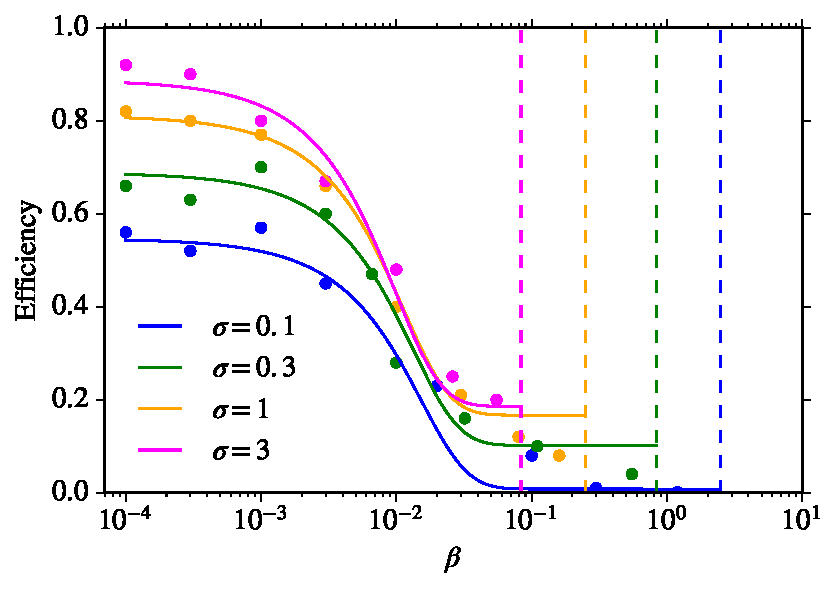
\includegraphics[width =\textwidth]{efficiency_fit.pdf}
\caption{Electron non-thermal acceleration efficiency $\epsilon$ as a function of $\beta$ (horizontal axis) and for different values of $\sigma$ (different colors, as indicated in the legend). The solid lines show our empirical fit in Equation \ref{fiteff}. For each $\sigma$, the solid lines extend up to maximum allowed $\beta$, i.e., $\beta_{\rm max}=1/4\sigma$.}
\label{efficiency_fit}
\end{figure}



\section{Electron Acceleration Mechanisms}\label{mechanism}
In order to understand the dependence on $\beta$  of the electron spectrum as discussed in the previous Section, it is instructive to investigate the physics of electron acceleration in our simulations.  To this end, we follow individual trajectories of the highest energy electrons in order to identify where they gain most of their energy and what are the physical processes responsible for their acceleration. We focus here on a few representative high-energy electrons. In a forthcoming paper, we will explore the physics of electron acceleration in greater detail.

We show in Figures \ref{lowbeta_prtl} and \ref{highbeta_prtl} the trajectories of two representative electrons. The former refers to a low-$\beta$ case with $\beta=3\times 10^{-4}$ and $\sigma=0.3$ (here, the high-energy electron belongs to the main component of particles accelerated by reconnection), while the latter refers to a high-$\beta$ case with $\beta=0.16\approx \beta_{\rm max}$ and $\sigma=1$ (here, the high-energy electron belongs to the additional component appearing when $\beta\approx \beta_{\rm max}$).

In Figures \ref{lowbeta_prtl} and \ref{highbeta_prtl}, the vertical axis represents time, in units of the Alfv\'en crossing time $t_A$. The background color in panel (a) shows the space-time diagram of  particle density. At each time, a 1D slice of density is extracted at $y=0$ (i.e., along the plane of the current sheet), and plotted as a function of $x$ (horizontal axis). The temporal evolution of the particle $x$-location is overplotted with a sequence of points, whose color corresponds to its energy (from cyan at the initial time, to pink at the final time). In panel (b), the orange line presents the time evolution of the particle $y$-position. Its first interaction with the current sheet (i.e., at $y=0$) is marked with the dashed horizontal line. Note that the $x$-position of the particle depicted in panel (a) can be meaningfully compared with the background density only when the particle $y$-coordinate in panel (b) is small (i.e., the particle is in the vicinity of the plane $y=0$ of the reconnection layer, where the density slices in panel (a) are taken).
In panel (c), we show the electron Lorentz factor $\gamma$. 
 In panel (d), we plot the temporal evolution of the quantity $E_{z}/\beta_{A}B_{xy}$ measured at the particle location, i.e., the out-of-plane electric field $E_z$ divided by the product of the in-plane magnetic field $B_{xy}=(B_{x}^{2}+B_{y}^{2})^{1/2}$ and the dimensionless Alfv\'en velocity $\beta_A=\sqrt{\sigma/(1+\sigma)}$. This will prove to be a useful diagnostic of the particle acceleration mechanisms, for the following reason: reconnection outflows move at roughly the Alfv\'en speed, so the motional electric fields carried by a magnetic field $B_{xy}$ are expected to be $E_{z,\rm ideal}\sim \beta_{A}B_{xy}$, in ideal MHD. On the other hand, in regions of strong magnetic dissipation  (e.g., at  X-points), non-ideal electric fields can largely exceed the MHD expectation, i.e., $E_z\gg E_{z,\rm ideal}$. It follows that when the ratio $E_{z}/\beta_{A}B_{xy}$ exceeds unity, it is likely that the particle is experiencing a strong non-ideal electric field, which can serve as an efficient particle accelerator.
   

\begin{figure*}[!t]
\centering
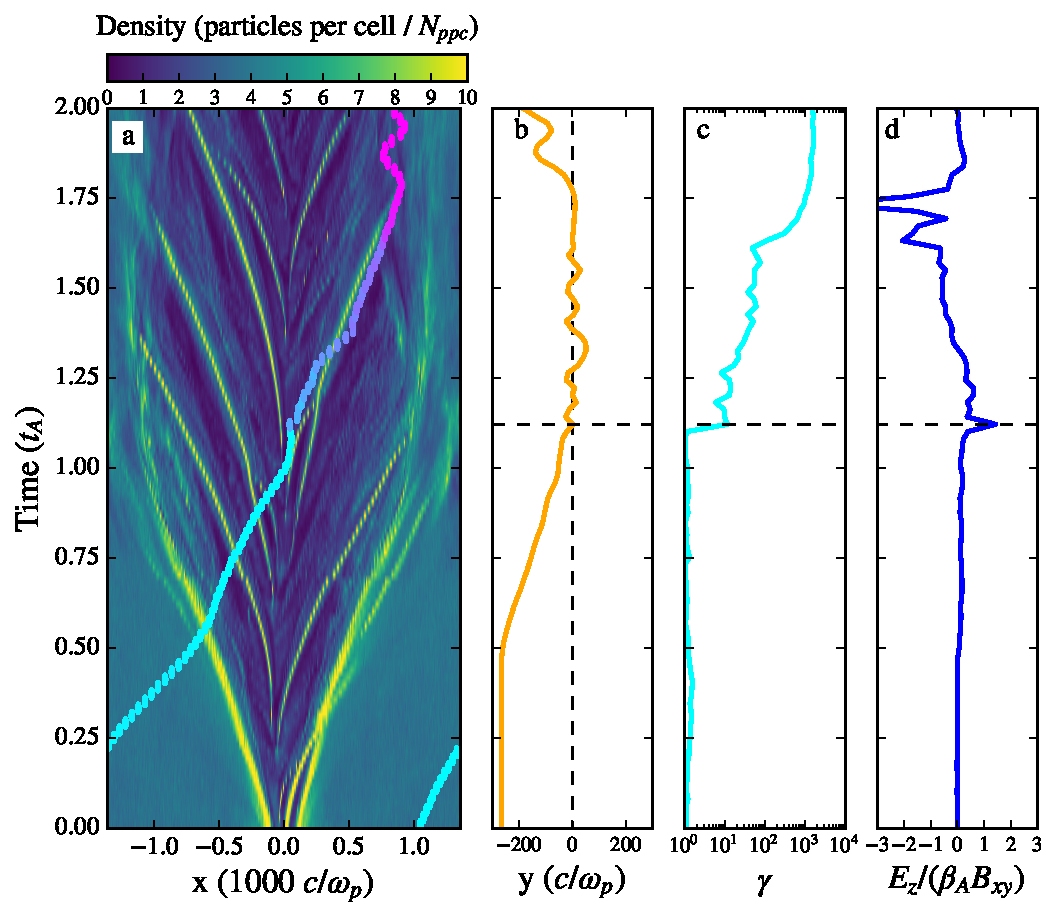
\includegraphics[width =\textwidth]{lowbeta_lec.pdf}
\caption{Representative electron trajectory from a simulation with $\sigma=0.3$ and $\beta=3\times 10^{-4}$ (simulation B1), whose temporal evolution of particle density and energy spectra is presented in  Figures \ref{lowbeta_threeplot} and \ref{timespec}, respectively. The vertical axis represents time in units of the Alfv\'en crossing time $t_A$.
The background color in panel (a) shows the space-time diagram of  particle density, composed of a sequence of 1D slices taken at $y=0$ (i.e., along the plane of the current sheet). The temporal evolution of the particle $x$-location is overplotted with points, whose color corresponds to the electron energy (from cyan at the initial time, to pink at the final time). In panel (b), the orange line presents the time evolution of the particle $y$-position. Its first interaction with the current sheet is marked with the dashed horizontal line. In panel (c), we show the electron Lorentz factor $\gamma$.  In panel (d), we plot the temporal evolution of the quantity $E_{z}/\beta_{A}B_{xy}$ measured at the particle location, which proves to be a useful diagnostic of the particle acceleration mechanisms. We find that the electron (and in general, all the high-energy electrons in low-$\beta$ runs) is accelerated by non-ideal electric fields at X-points, either in the main layer, or in current sheets formed during plasmoid mergers.}
\label{lowbeta_prtl}
\end{figure*}

%%%%%%%%%%%%%
\subsection{Electron Acceleration at Low $\beta$}
We show in Figure \ref{lowbeta_prtl} a representative high-energy electron extracted from a simulation with $\sigma=0.3$ and $\beta=3\times 10^{-4}$. For this case, we have presented the temporal evolution of the particle density in Figure \ref{lowbeta_threeplot} and of the electron and proton energy spectra in Figure \ref{timespec}.

A comparison of panel (b) and (c) demonstrates that the electron is first accelerated when it interacts with the current sheet for the first time (i.e., at the time marked by the horizontal dashed line). During this first interaction with the layer, the particle experiences a value of $E_{z}/\beta_{A}B_{xy}$ larger than unity (panel (d)), indicating that acceleration is driven by non-ideal electric fields. In fact, panel (a) shows that during this acceleration episode the electron is located in one of the under-dense regions associated with X-points. Accelerated by the non-ideal electric field, the electron Lorentz factor at the X-point quickly increases from $\gamma\approx 1$ up to $\gamma \approx 20$ (panel (c)).

The electron is then trapped in a secondary plasmoid, which can be identified in panel (a) as the yellow structure that the particle orbit follows at $1.2\lesssim t/ t_A\lesssim 1.7$. While in the plasmoid, the electron energy stays nearly constant, aside from a moderate increase (by roughly a factor of two) when the electron moves from the trailing to the leading edge of the plasmoid at $t\simeq 1.3\, t_A$. 

At $t\simeq 1.7\, t_A$, when the plasmoid merges with the boundary island, the electron lies in between the two. At the interface of the two  merging structures, a current sheet forms along the $y$ direction, i.e., perpendicular to the main reconnection layer (e.g., see the interface at $x\approx -1500 \, c/\omega_{p}$ in Figure \ref{lowbeta_threeplot}(c)). As it happens for the main layer, the newly developed current sheet breaks into a series of secondary plasmoids separated by X-points. At one of such X-points, the non-ideal electric field further increases the electron energy up to  $\gamma \approx 10^3$. The role of the non-ideal electric field is revealed in panel (d) by the peak with $E_{z}/\beta_{A}B_{xy}\lesssim -2$ at $t\simeq 1.7\, t_A$. Its sign is consistent with the fact that the non-ideal electric field in between merging plasmoids is expected to have opposite direction than in the main layer (i.e., it is oriented along $-\bm{\hat{z}}$ rather than $+\bm{\hat{z}}$). 

While many low-$\beta$ electron trajectories resemble the one we have presented here, some electrons show only one episode of acceleration, analogous to either the first or the second stage shown in Figure \ref{lowbeta_prtl}. In other words, 
some electrons pick up all of their energy at an X-point during their first interaction with the current sheet (either at the primary X-point or at one of the secondary X-points), while others are accelerated at current sheets formed when secondary plasmoids merge with each other or with the boundary island.  In either case, in low-$\beta$ simulations all the high-energy electrons are predominantly accelerated by non-ideal electric fields associated with reconnecting magnetic fields, either at the primary X-point, at secondary X-points, or in current sheets formed during plasmoid mergers.


\begin{figure*}[!t]
\centering
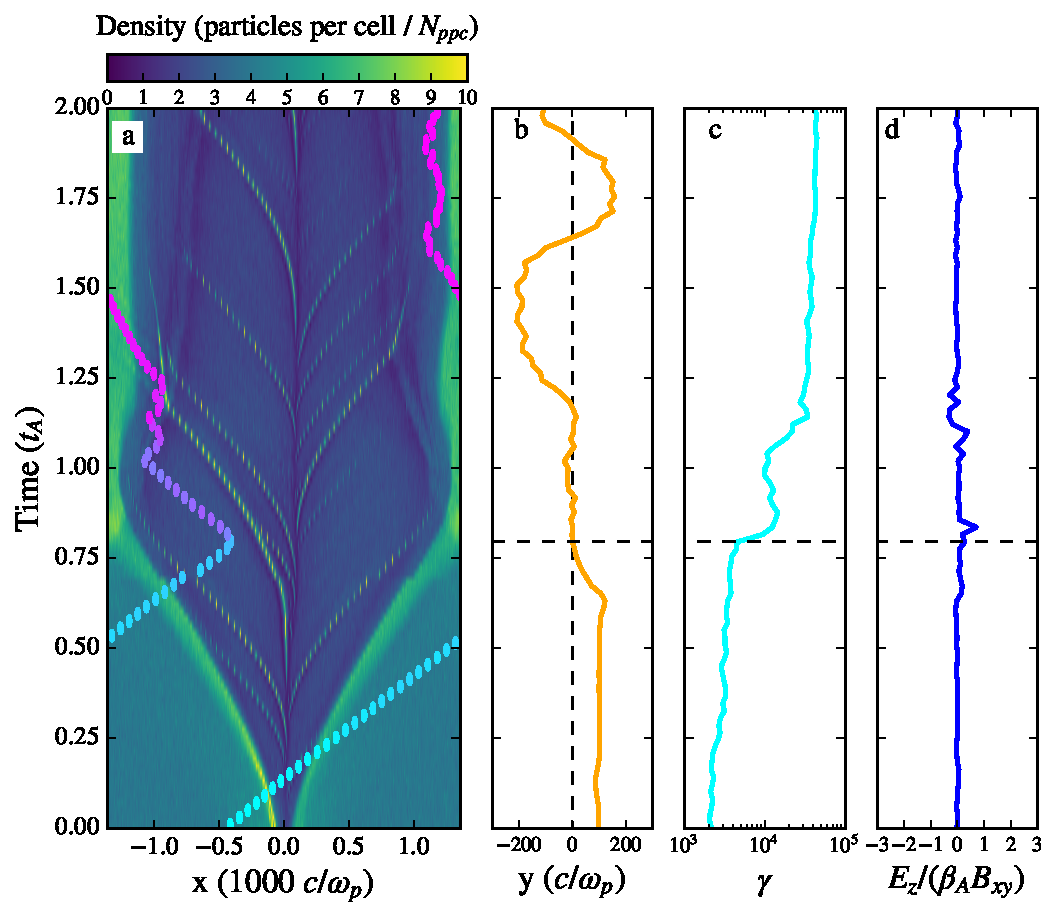
\includegraphics[width =\textwidth]{highbeta_lec.pdf}
\caption{Electron trajectory from a simulation with $\sigma=1$ and $\beta=0.16$ (simulation C7), as a representative case of particles (both electrons and protons) belonging to the additional high-energy component appearing for $\beta\approx \beta_{\rm max}$. The temporal evolution of the corresponding electron energy spectrum is shown in Figure \ref{sig1_timespec}. See Figure \ref{lowbeta_prtl} for a description of the content of the panels.  We find that most of the particle energy gain comes from a Fermi-like process, while the electron is bouncing between the reconnection outflow and the edge of the boundary island.}
\label{highbeta_prtl}
\end{figure*}


\subsection{Electron Acceleration at $\beta\approx \beta_{\rm max}$}
We show in Figure \ref{highbeta_prtl} the trajectory of a representative electron from a simulation with $\sigma=1$ and $\beta=0.16$. This is the simulation that shows the strongest signature of the additional high-energy component appearing at late times for $\beta\approx \beta_{\rm max}$. The temporal evolution of the corresponding electron spectrum is shown in Figure \ref{sig1_timespec}.

Two phases of energization are seen in the time evolution of the electron energy (panel (c)). The first one (with an increase in Lorentz factor from $\gamma \approx 2\times 10^3$ up to $\gamma \approx 10^4$) is associated with the first encounter with the current sheet (as marked by the horizontal dashed line), in a similar way as we have discussed above for the low-$\beta$ case. However, the electron in  Figure \ref{highbeta_prtl} interacts with the unstructured outflow, and not with an X-point (see panel (a)). As a result, the value of $|E_{z}|/\beta_{A}B_{xy}$ along the electron trajectory (panel (d)) is much smaller than in the low-$\beta$ case. Most of the inflowing electrons experience this acceleration episode at their first encounter with the current sheet, regardless of where they interact. So, unlike in the low-$\beta$ case, they do not need to enter the layer at an X-point in order to be accelerated. Since such an energization phase is common to the majority of electrons, it should be regarded as bulk heating, rather  than non-thermal particle acceleration. In fact, an electron with $\gamma \approx 10^4$ (as appropriate for the electron in Figure \ref{highbeta_prtl}, after the first energization episode) would not belong to the high-energy spectral component seen in Figure \ref{sig1_timespec} (that lies at $\gamma\gtrsim 2\times 10^4$). 

After it reaches the outskirts of the boundary island at $t\simeq t_A$, the electron is  accelerated up to $\gamma \approx 7\times 10^4$ (so, well within the energy range covered by the high-energy component in Figure \ref{sig1_timespec}).  From $t\simeq t_A$ to $t\simeq1.2\, t_A$, it stays confined between the boundary island and the reconnection outflow. We attribute the energy increase in this phase (panel (c)) to a Fermi-type process in between converging flows (i.e., the reconnection outflow and the boundary island), for two main reasons: (\textit{i}) as in the first phase of energization, this second episode does not arise from a strong non-ideal electric field (panel (d)), as it would rather be expected for X-point acceleration; (\textit{ii}) the fractional energy gain is comparable between the first and second phases of energization, as expected for a Fermi-like process (see the next Subsection).

We find that all of the highest energy electrons in $\beta\approx \beta_{\rm max}$ simulations show this Fermi-type acceleration as they get trapped between the reconnection outflow and the boundary island. Also,  the highest energy protons in  $\beta\approx \beta_{\rm max}$ simulations display the same acceleration physics as electrons, which explains the similarity between the energy spectra of the two species (compare red and cyan lines in Figure \ref{sig1_timespec}).

%The dominant acceleration mechanisms present in this high-$\beta$ simulation seems to be more similar to shock acceleration, where particles are sampling convergent velocity fields across overdense regions (the outflow and boundary island), rather than x-point acceleration, where electrons are accelerated by non-ideal electric fields in underdense environments (x-points).

%In order for particles to sample the velocity difference between the outflow and the island, they must have Larmor radii that are on the same scale as the velocity convergence, which will be on proton scales (i.e., $\sim$ 1 proton skin depth).  The Larmor radius of an electron in units of the proton skin depth is
%\begin{equation}
%\frac{\rho_{e}}{d_{i}} = \gamma_{e}\frac{v_{e}}{c}\frac{m_{e}}{m_{i}}\frac{1}{\sqrt{\sigma_{i}}}.
%\end{equation}
%Considering the high-$\beta$ electron we show in Figure \ref{highbeta_prtl}, we see that after the electron's first interaction with the current sheet, it has a Lorentz factor of roughly $10^{4}$.  At this point, the electron's Larmor radius is $\approx$ 3.5, large enough for the electron to sample velocity convergence between the outflow and the boundary island, and receive another boost in energy, up to its final value of $\gamma \approx 10^{5}$.



\subsection{Comparing the Acceleration Mechanisms}
In this Subsection, we present a few qualitative arguments to justify why X-point acceleration plays a more significant role at low $\beta$, whereas the Fermi process is predominant at high $\beta$ (and more specifically, at $\beta\approx \beta_{\rm max}$). We defer a more detailed analysis of the physics of particle acceleration to a future study.

First, as shown in Figures \ref{sig_3_twoplot} and \ref{sig3_twoplot}, low-$\beta$ simulations display a much higher number of secondary plasmoids (and consequently, of secondary X-points) than high-$\beta$ runs. It follows that the fraction of inflowing electrons that are likely to enter the current sheet at the location of an X-point --- where they can be accelerated by non-ideal electric fields --- is higher at lower $\beta$, resulting in higher acceleration efficiencies.

Second, the strength of the reconnection electric field $E_z$ is proportional to the particle inflow rate (i.e., to the reconnection rate), which steadily decreases as $\beta$ increases (at fixed $\sigma$), as shown in Figure \ref{inflow_rates_over_Va}. So, the non-ideal electric field will be weaker at higher $\beta$, resulting in a slower rate of particle acceleration at X-points.

Finally, we can compare the typical energy gains expected from one episode of X-point acceleration and one Fermi cycle, as a function of $\sigma$ and $\beta$. The electron energy gain at an X-point will equal the work performed by the non-ideal electric field, which we set to be a fraction $\sim 0.1\,\beta_{A}$ of the upstream magnetic field $B_0$. So,
\begin{equation}
\Delta\gamma_{e,\rm X} m_{e} c^{2} \approx  0.1 \beta_{A} e B_{0} L~,
\end{equation}
where $L$ is the length of the acceleration region in the $z$-direction. If $L$ is normalized to the proton skin depth, with $L=L_{di} \,c/\omega_{pi}$, we find
\begin{equation}\label{xpoint-gain-temp}
\Delta \gamma_{e,\rm X} \approx  0.1 \frac{m_{i}}{m_{e}} \frac{\sigma}{\sqrt{\sigma+1}} L_{di}~.
\end{equation}
Clearly, the energy gain for X-point acceleration is insensitive to the initial electron temperature. On the other hand, the fractional energy increase per Fermi cycle is $\sim \beta_A$, if particles bounce between the reconnection outflow (which is moving at $\sim v_A$) and the boundary island (which is stationary).\footnote{We are also implicitly assuming that the converging flows are non-relativistic, which requires $\sigma\lesssim 1$ (so that the Alfv\'en speed is non-relativistic).} It follows that
\begin{equation}\label{fermi}
\Delta \gamma_{e,\rm Fermi}\approx \beta_A \theta_e~,
\end{equation}
and if protons and electrons are set up in temperature equilibrium, 
\begin{equation}\label{fermi}
\Delta \gamma_{e,\rm Fermi}\approx \beta \frac{m_i}{m_e} \frac{\sigma^{3/2}}{\sqrt{\sigma+1}}~.
\end{equation}
% We can infer the typical values of $L_{di}$ from the typical energy gains we see in our simulations.  For the low-$\beta$ trajectory we show, the electrons are typically energized to $\gamma\approx 100$ or $1,000$ at an x-point.  This implies $L_{di}$ of around 2 to 20.
This simple argument shows that, for fixed $\sigma$, X-point acceleration will provide a larger energy gain at low $\beta$, whereas the Fermi process will be energetically dominant in the high-$\beta$ regime.



%Considering the relativistic limit of this, where Fermi acceleration will dominate over x-point acceleration, because the electrons are starting out very hot,

%\begin{equation}
%\frac{\rho_{e}}{d_{i}} \approx 3 \theta_{i} / \sqrt{\sigma}.
%\end{equation}
%Plugging in typical values of a high-$\beta$ simulation ($\sigma=1$, $\theta=0.2$), we get $\rho_{e}/d_{i} \approx 0.6$, which is about the width of the reconnection outflow.  As the temperature decreases, the electrons will become increasingly tied to the magnetic field lines and not be able to sample the large-scale velocity differences in the outflow and between plasmoids. 

%We can make an estimate for the typical $\theta$, at which Fermi reflection becomes dominant
%We can estimate the typical $\theta$, and hence, $\beta$ that the transition from x-point to Fermi acceleration is dominant,
%\begin{equation}
%\theta_{crit} = 0.1 L_{di} \sqrt{\sigma}
%\end{equation}
%in the non-relativistic case, and 
%\begin{equation}
%\Delta E / E_{0} \approx (v_{A}/c)^{2}
%\end{equation}
%in the relativistic case.  



%Additionally, if an electron interacts with an x-point, the energy gain provided by the electric field will be a smaller fraction of the initial particle energy as $\beta$ increases, while the energy gain from a Fermi-type process is directly proportional to the particle's initial energy.  This indicates that Fermi-type processes will be energetically dominant over x-point acceleration for hotter plasmas.

%Finally, we can make a simple estimate of how much energy is picked up by a particle passing through an x-point, and examine how this quantity depends on the plasma-$\beta$.  Consider a particle with a velocity in the x-y plane given by $v_{th}$.  Imagine that this particle passes through a region with constant electric field $E_{z}$, and this region has a width of $W$.  The particle's kinetic energy will change by
%\begin{equation}
%\Delta T = \int_{}^{}\vec{F} \cdot \vec{dl} =q E_{z}\Delta z.
%\label{delta_T}
%\end{equation}
%$\Delta z$ will be set by the amount of time the particle spends in the acceleration region, $t_{acc} = W/v_{th}$, and the average z-velocity.  Because we assume a constant acceleration (constant $E_{z}$ in the x-point region), we can express the average z-velocity simply as $\bar{v_{z}}= v_{z, max}/2=t_{acc} q E_{z} / (2m)$.  As such, we get $\Delta z = t_{acc}^{2} q E_{z} / 2m $.  Plugging back into Equation \ref{delta_T}, we find:

%\begin{equation}
%\Delta T = \frac{q^{2} E_{z}^{2} t_{acc}^{2}}{2m} = \frac{q^{2}E_{z}^{2} W^{2}}{2 m v_{th} ^{2}} \approx \frac{q^{2}(V_{in} B_{0})^{2} W^{2}}{2 m v_{th} ^{2}}.
%\end{equation}
%Combining our constants into a single variable, C, and substituting in for the thermal velocity, we see that
%\begin{equation}
%\Delta T = \frac{CV_{in}^{2} B_{0}^{2} W^{2}}{KT}.
%\end{equation}
%note that $B_{0}^{2} / KT$ is proportional to $\beta^{-1}$ (for fixed density, $n$).  Based off of this simple, but physically motivated picture of particle acceleration via out-of-plane electric fields at x-points, we see that the energy gain of a particle is inversely proportional to the plasma-$\beta$ due to the fact that as particles stream through the x-point at faster thermal speeds, they will spend less time being accelerated by the $E_{z}$ fields, and hence not pick up as much energy.  This dependence on plasma-$\beta$ is likely even more drastic than $\beta^{-1}$, since there is a factor of $V_{in}^{2}$, which we have seen also depends on $\beta$, with $V_{in}$ decreasing with increasing $\beta$.  


\section{Conclusions}\label{conclusions}
In this work, we have investigated with large-scale 2D PIC simulations the physics of non-thermal particle acceleration in trans-relativistic  reconnection, covering the whole parameter space in $\sigma$ and $\beta$ and employing the physical proton-to-electron mass ratio. For four values of the magnetization ($\sigma=$ 0.1, 0.3, 1, and 3), we have explored a wide range of $\beta$, from $\beta=10^{-4}$ up to the maximum possible value of $\beta$, that is $\beta_{\rm max}\approx 1/4\sigma$. 


%In addition, our computational domains are larger than previous works by at least a factor of $\sim5$.

We find that the electron spectrum in the reconnection region can be generally modeled as a non-thermal power law, but the properties of the spectrum are strongly dependent on $\beta$. At $\beta \lesssim 3 \times 10^{-3}$, electron acceleration is efficient. The electron spectrum is dominated by a hard power law, whose slope is insensitive to $\beta$ and depends on $\sigma$ as $p\simeq 1.8 +0.7/\sqrt{\sigma}$, in agreement with the result by \citet{werner2018} (that employed a fixed $\beta=0.01$). The electron power-law tail tends to steepen for larger simulation domains. By tracking a large number of particles in our simulations, we find that at low $\beta$, electrons are primarily accelerated by the non-ideal electric field at X-points, either  in the initial current layer  or in current sheets generated in between merging magnetic islands. 


At higher $\beta$, the electron power law steepens significantly, and the electron spectrum eventually approaches a Maxwellian distribution, for all values of $\sigma$ (so, the efficiency of non-thermal electron acceleration drops). At high values of $\beta$ near $\beta_{\rm max}\approx1/4\sigma$, when both electrons and protons start relativistically hot, the spectrum of both species displays an additional component at high energies, containing a few percent of particles, which are accelerated via a Fermi-like process by bouncing in between the reconnection outflow and the stationary magnetic island at the boundary of our periodic domain.

For the main population of non-thermal electrons (i.e., excluding the additional component emerging at $\beta\rightarrow \beta_{\rm max}$),
we provide an empirical prescription for the dependence of the power-law slope and the acceleration efficiency on $\beta$ and $\sigma$. We also measure the inflow rate (i.e., the reconnection rate) as a function of $\beta$ and $\sigma$, and find that, for a given $\sigma$, the reconnection rate steadily decreases with increasing $\beta$.

Our results can provide a physically-grounded prescription for non-thermal electron acceleration via magnetic reconnection, in a regime relevant to hot accretion flows like Sgr A* at our Galactic center (e.g., \citealt{ball2016}; \citealt{mao2017}; \citealt{chael2017}). When implemented as subgrid models into global MHD simulations, our findings have the potential to unveil the origin of the flaring behaviour of Sgr A* \citep{ponti17}.
% Additionally, this study expands our understanding of magnetic reconnection in a regime that is just beginning to be explored, and shows the drastic effects that changing the plasma-$\beta$ has on the outcome of reconnection.  This study serves as an important first step towards building a fully physical model of electron acceleration in the trans-relativistic regime and highlights the important role that the plasma-$\beta$ plays in the final energy spectrum.

We conclude with a few caveats. In this paper, we have only considered reconnection setups with no guide fields and equal electron and proton temperatures.  However, for application to accretion flows around black holes, we generally expect non-zero guide fields in reconnection regions (\citealt{ball2017}), and protons to be significantly hotter than electrons.  Also, we have employed 2D simulations, and one might argue that 3D effects may alter the physics of electron acceleration and the resulting electron energy spectra.
 We will explore these effects in future studies.






\section{Appendix A: Dependence on Box Size}\label{boxsize}
To test the effect of box size on our results, we perform simulations with varying box size for a number of combinations of $\sigma$ and $\beta$.  Previous studies (e.g., \citealt{werner2018}) have shown that both the power-law slope and high-energy cutoff of the electron energy spectra increase with increasing box size (i.e., at the box size increases, the spectra become steeper, but extend to higher energies).  \citet{werner2018} probed box sizes from $20-120 \; \rho_{c}$, where $\rho_{c}$ is the Larmor radius of an electron with energy $\sigma_{e}$.  The precise reason for this dependence is not yet understood.  To this end, we aim to explore how the power-law index and high-energy cutoff depend on box size in our simulations. We perform our tests for box size both at low-$\beta$, as well as in a high-$\beta$ case, which displays a second component in its spectrum.  

We show in Figure \ref{sigpoint3_boxsize} electron spectra for simulations with $\sigma=0.3$ and $\beta=0.006$, across five different box sizes, defined by the number electron skin depths along the current sheet, at values of 680, 1,360, 2,720, 5,440, and 10,880 (corresponding to 73.6, 147.2 294.5, 589, and 1,178 $\rho_{c}$).  In order to directly compare the spectra at varying box sizes, we normalize the spectra by a factor proportional to $(L_{x}^{2}$, which makes it such that there are roughly the same number of particles in the reconnection region.  We see that there is a trend of the slope increasing with increasing box size, shown in the inset of Figure \ref{sigpoint3_boxsize}.  We find that the slopes begin to level out towards our largest boxes, but note that the inset's scale is log-linear: the slope's dependence on box size is quite weak.  Additionally, we see evidence of the high-energy cutoff increasing with box size.


\begin{figure}[!h]
	\centering
	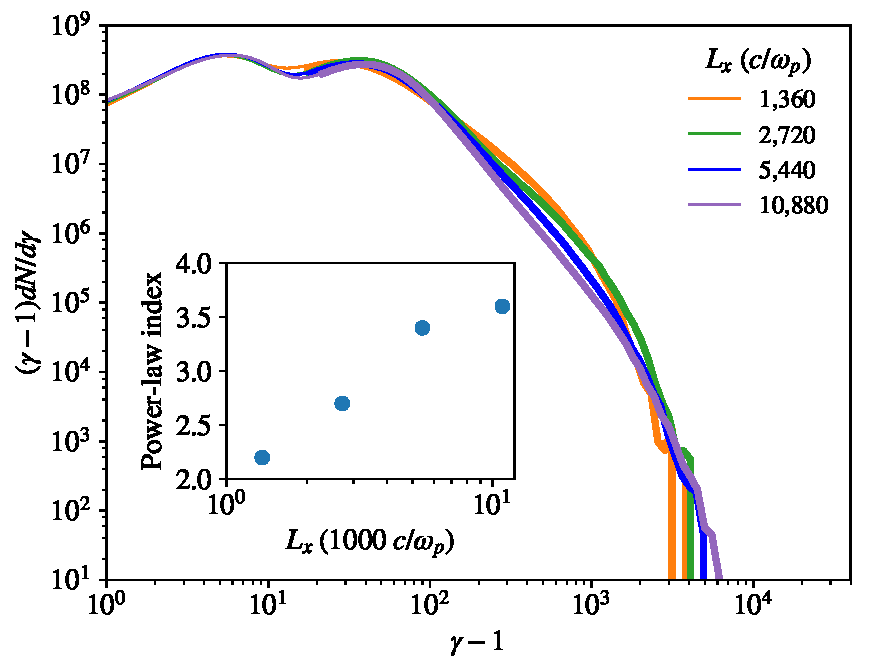
\includegraphics[width =0.75\textwidth]{sig_3_delgam001_boxsize.pdf}
	\caption{Electron spectra for $\sigma=0.3$, $\beta=0.006$, taken at $t\approx 2t_{A}$ across five different box sizes, defined by the number of cells in the direction along the current sheet (x-direction). Inset: Power-law index as a function of boxsize for the spectra shown: as the box length increases, that the power-law index gets larger.}
	\label{sigpoint3_boxsize}
\end{figure}


We also show the spectra's trend with box size for a simulation with $\sigma=1$ and $\beta=0.16$ in Figure \ref{sig1_boxsize}, a case with the extra high-energy component for our fiducial box size of 5,440 skin depths along the current sheet.  The kink in the spectra at high-energies becomes more prominent towards larger boxes: in the $L_{x}=1,360 \; c/\omega_{p}$ (orange) box, there is no notable signature of the slope hardening at high-energies. In the $L_{x}=2,720$ (green) the spectra begins to kink, and at 5,440, there's a definitive hardening in the slope just above $\gamma=10^{4}$, which persists to $\approx 10^{5}$.  Extending to even larger boxes than our fiducial case of 5,440, the feature becomes even more prominent.  We see the cutoff energy of this feature increasing (roughly linearly) with box size.  This emphasizes the importance large simulation domains in unveiling the physics of trans-relativistic magnetic reconnection.




\begin{figure}[t]
\centering
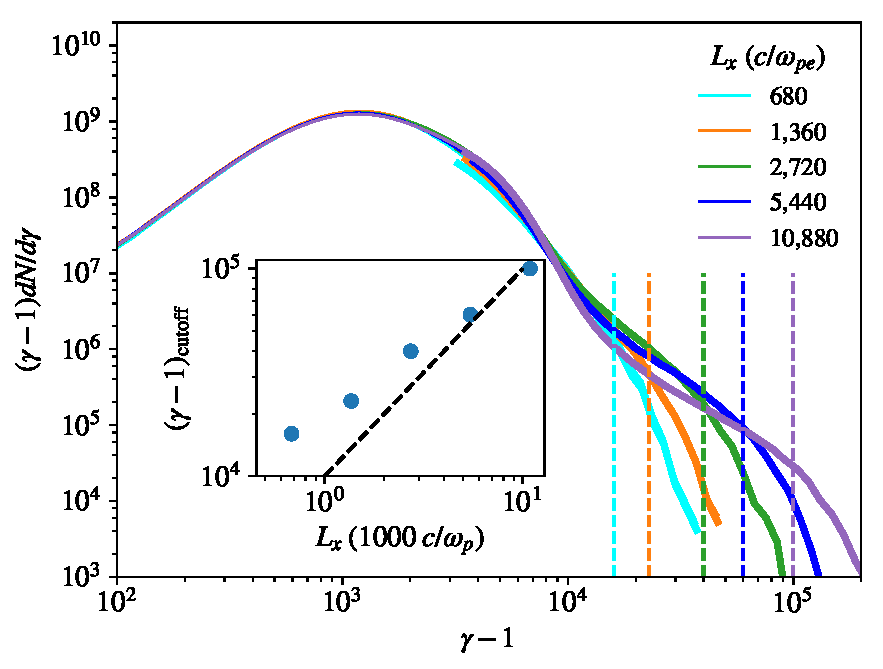
\includegraphics[width =0.75\textwidth]{sig1_delgam_2_boxsize.pdf}
\caption{Electron spectra for $\sigma=1$, $\beta=0.16$ across 5 different box sizes, taken at $t\approx 2t_{A}$.  The kink in the spectra only emerges towards larger boxes, becoming most prominent in our 16k box.  We show our estimates for the high-energy cutoff, the point at which a power-law like tail begins to exponentially fall off, with dashed horizontal lines.  The inset shows the cutoff energy as a function of box size (blue circles), while the dashed black line depicts a slope of unity for reference.}
\label{sig1_boxsize}
\end{figure}

\section{Appendix B: Boundary Conditions and Triggering Mechanisms}\label{untriggered}
In our fiducial simulations, we trigger reconnection at the center of the box and employ periodic boundary conditions in the x-direction (along the current sheet).  In this appendix, we explore the effects of these choices.  To this end, we run simulations with outflowing boundary conditions along the x-direction, as well as simulations where reconnection evolves spontaneously from noise, with no imposed triggering mechanism.  For the untriggered simulations, we employ thinner current sheets ($\Delta=20$ cells) so that the tearing instability will set in quickly.  For the outflow conditions, the setup of the current sheet is identical to the triggered simulations.

We show in Figures \ref{sigpoint3_outflow_early}-\ref{sig1_outflow_early} the spectra of three simulations at early and late times.  The spectra depicted in these figures are all from simulations with $\sigma=0.3$ and $\beta=0.006$.  The untriggered periodic, triggered periodic, and triggered outflow simulations correspond to the orange, cyan, and purple lines, respectively.  We show in the top panel of Figure \ref{sigpoint3_outflow_early}, spectra from a time before the reconnection fronts have reached the boundary in the triggered simulations.  We see at this early time that the spectra from the triggered outflow and periodic simulations are identical.  This is expected, since the outflowing plasma has not yet reached the boundaries, so the differing boundary conditions have not yet influenced the spectra.  The untriggered spectrum, however, shows a significantly harder spectrum.  In the bottom panel of the same figure, we show the spectra from the same simulations at a later time, once reconnection has halted in the periodic simulations due to finite box size and influence of the boundaries.  We see that the untriggered spectrum is still significantly harder than the triggered periodic (our fiducial choice) simulation: we measure a power-law index of 2.7 for the untriggered electron energy spectrum, while the corresponding simulation's electron energy spectra has a power-law index of 3.4.  The significantly harder electron spectrum in the untriggered case may be due to the fact that, for an untriggered simulation, the initial current layer will break up into numerous primary x-points, which may serve as sites of electron acceleration in low-$\beta$ reconnection (see, e.g., section 6.1).  In the triggered simulations, however, because we trigger the local collapse of the current sheet, there is only one primary x-point.  Additionally, in the case of untriggered reconnection, there are many more equal-sized plasmoid mergers, since the final magnetic island is assembled through the hierarchical merging of the initial plasmoids.  In contrast, in the triggered simulations, when secondary plasmoids form, they are quickly pulled towards the edge of the box, which suppresses their tendency to hierarchically merge with other plasmoids of similar sizes to build large plasmoids in the current layer, and accelerate particles during these mergers.  While these are plausible explanations for why the untriggered electron spectra are significantly harder than the triggered cases, we defer a detail physical analysis of this phenomenon to future work.  We see that the outflow simulation shows a slightly harder slope than the triggered periodic case at late times.  This may be due to some degree of thermalization that occurs when secondary plasmoids merge into the boundary island, which would then build up a larger thermal peak for periodic systems, but we defer a more thorough examination of this to future work.

\begin{figure}[!h]
	\centering
	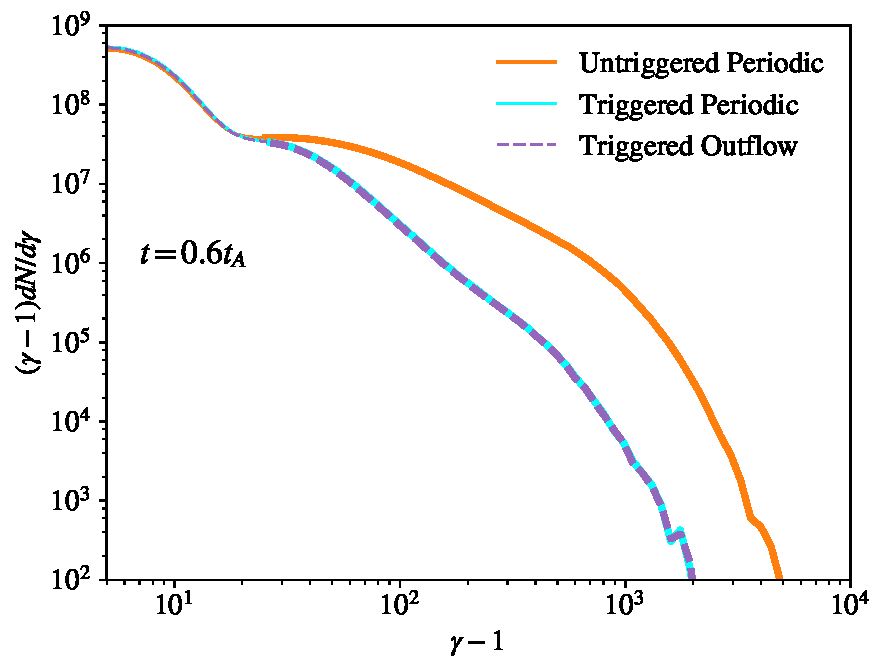
\includegraphics[width =0.75\textwidth]{sig_3_delgam001_outflow_untriggered_earlytime.pdf}
	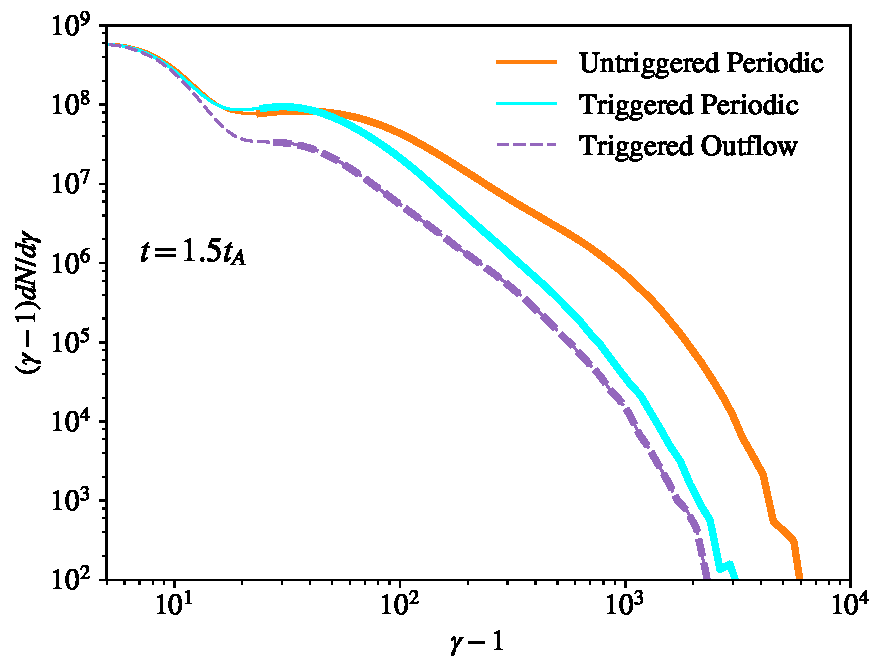
\includegraphics[width =0.75\textwidth]{sig_3_delgam001_outflow_untriggered_latetime.pdf}
	\caption{Electron spectra for simulations with $\sigma=0.3$, $\beta=0.006$ at 0.5 (top) and 2 (bottom) Alfv\'en crossing times.  The fiducial triggered and periodic simulation is shown in red.  The triggered outflow, and untriggered periodic simulations are shown in purple and orange, respectively.  In the top panel (early time), boundary effects have not yet influenced the spectra, and the two triggered simulations with periodic and outflow boundaries are identical.  The untriggered simulation, however, shows a significantly harder spectra.  At a later time (bottom), the boundaries affect the spectra and the triggered periodic simulation shows a softer slope than the triggered outflow.}
	\label{sigpoint3_outflow_early}
\end{figure}
We show plots analogous to the previous two in Figure \ref{sig1_outflow_early}, but for simulations with $\sigma=1$ and $\beta=0.16$.  We aim to see whether the extra component is due to the choice of triggering mechanisms, or it is a general feature of high-beta reconnection in large enough boxes.  We once again see that at early times (top panel of Figure \ref{sig1_outflow_early}), the triggered outflow and periodic spectra are identical, while the untriggered simulation shows a harder high-energy spectrum.  At late times (bottom panel), we see that there is a kink in the spectra of both the untriggered and triggered periodic simulations, where the spectra become harder, and extend to high energies.  While the precise characteristics of this additional component are different between the triggered and untriggered simulations, we do indeed find that it is a general feature of high-$\beta$ reconnection for large periodic systems.  In the outflow case, we do not see the signature of this feature.  This is likely due to the fact that this feature is associated with regions of strong velocity convergence, which are absent in the outflow simulations.



%\begin{figure}[!h]
%\centering
%\includegraphics[width =0.5\textwidth]{sig_3_delgam001_outflow_untriggered_spect_latetime.png}
%\caption{Electron spectra for simulations with $\sigma=0.3$, $\beta=0.006$, shown at an Alfv\'en crossing time of $\approx2$.  At this point, a significant amount of plasma has left the system in the outflowing simulation.  .The untriggered simulation shows a significantly harder spectra.}
%\label{sigpoint3_outflow_late}
%\end{figure}



\begin{figure}[!h]
\centering
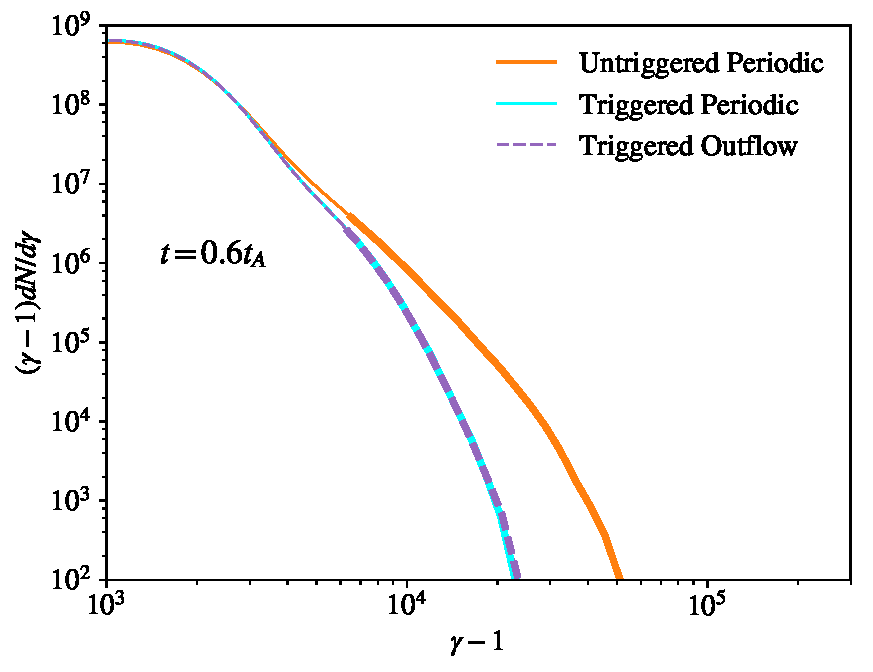
\includegraphics[width =0.75\textwidth]{sig1_delgam_2_outflow_untriggered_earlytime.pdf}
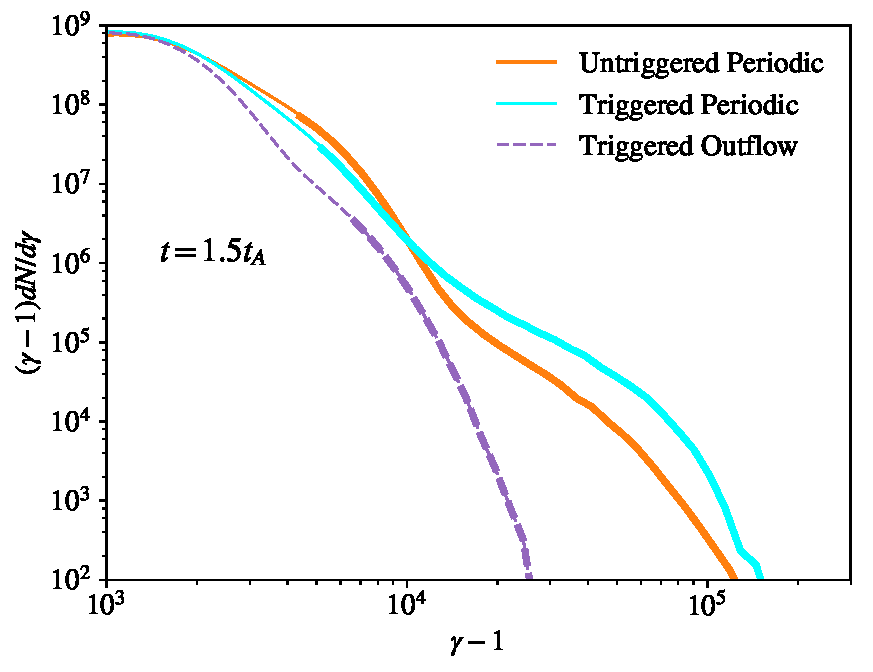
\includegraphics[width =0.75\textwidth]{sig1_delgam_2_outflow_untriggered_latetime.pdf}
\caption{Electron spectra for simulations with $\sigma=1$, $\beta=0.16$, shown at an Alfv\'en crossing time of $\approx0.5$ (top) and $approx 2$ (bottom).}
\label{sig1_outflow_early}
\end{figure}


%\begin{figure}[!h]
%\centering
%\includegraphics[width =0.5\textwidth]{sig1_delgam_2_outflow_untriggered_spect_latetime.png}
%\caption{Electron spectra for simulations with $\sigma=1$, $\beta=0.16$, shown at an Alfv\'en crossing time of $\approx2$.  We see that the high-energy kink in the spectrum emerges in both the triggered and untriggered simulations.}
%\label{sig1_outflow_late}
%\end{figure}


\section{Appendix C: Convergence tests}\label{convergence}
To ensure that our results are not being affected by our choice in the initial number of particles per cell ($N_{ppc}$) we employ, or the resolution, we perform simulations where we significantly increase these quantities.  In Figure \ref{ppc_spect}, we show the results of quadrupling the initial number of particles per cell, from our fiducial value of 4.  We find that increasing this quantity has little to no effect on the spectra.  

\begin{figure}[!h]
\centering
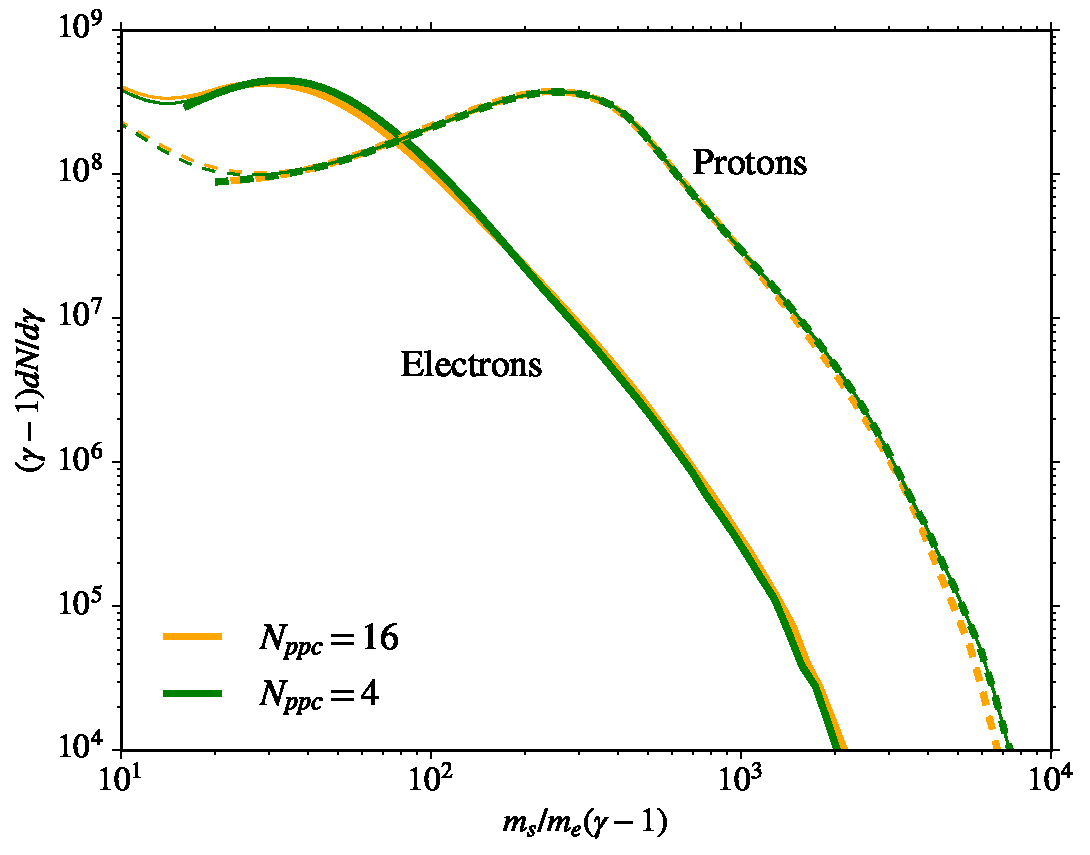
\includegraphics[width =0.75\textwidth]{ppc_final.pdf}
\caption{Electron (solid) and proton (dashed) energy spectra for simulations with $\sigma=0.3$, $\beta=0.006$, with $N_{ppc}=4$ (green) and $N_{ppc}=16$ (orange).  Spectra are computed at $t\approx 2t_{A}$  We see very little difference between the spectra from these two simulation, despite quadrupling the initial number of particles per cell.}
\label{ppc_spect}
\end{figure}

We also run a simulation where we double the spatial resolution (from our fiducial value of three cells per electron skin depth, to six), in order to ensure that our results are not sensitive to increasing the resolution.  This high-resolution simulation has the same physical box size in electron skin depths, and is compared to the fiducial run when the simulations are at equal light crossing times.  We show the electron and proton spectra in the reconnection region for these two simulations in Figure \ref{comp_spect}.  We see that the high energy slope of the electrons is unchanged, despite doubling the resolution.

\begin{figure}[!h]
\centering
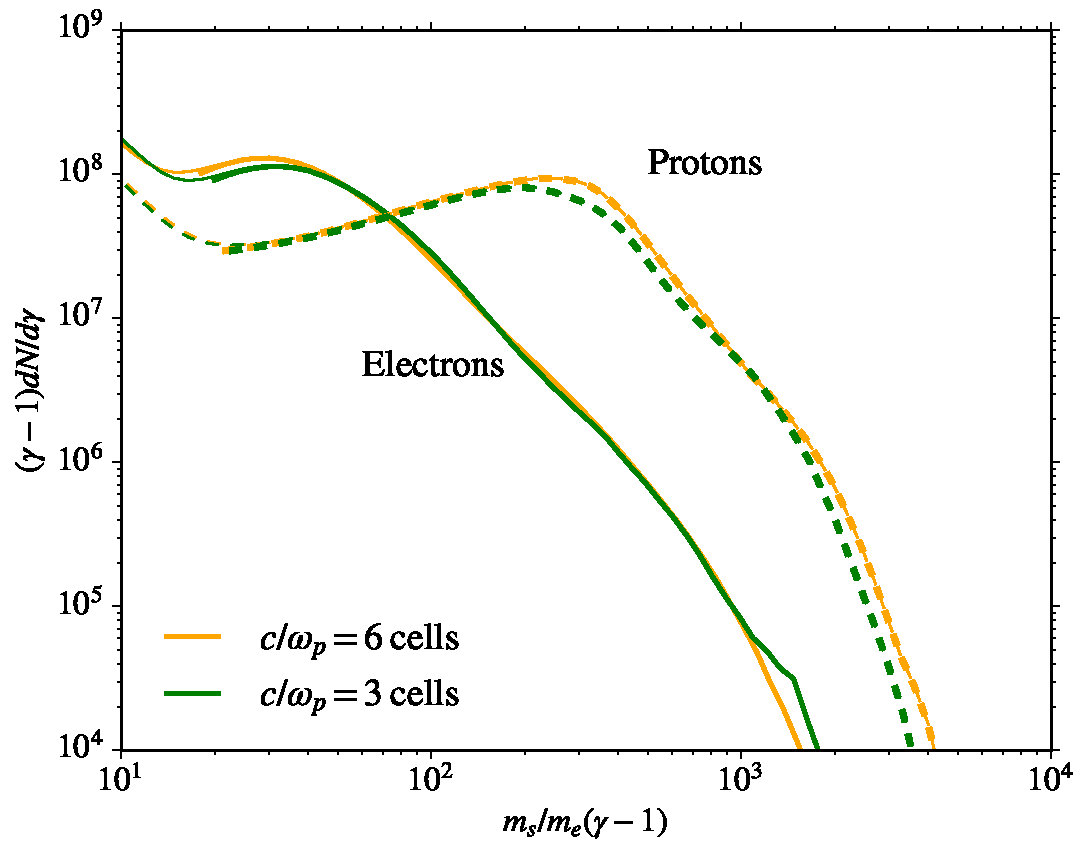
\includegraphics[width =0.75\textwidth]{comp_final.pdf}
\caption{Electron (solid) and proton (dashed) energy spectra for simulations with $\sigma=0.3$, $\beta=0.006$, where an electron skin depth is resolved in 3 (green) and 6 (orange).  Spectra are computed at $t\approx 2t_{A}$  }
\label{comp_spect}
\end{figure}


\section{Appendix D: Decomposing the Particle Spectra}\label{shells}
In order to investigate the detailed structure of the electron energy distribution and how it may change throughout the boundary island, we decompose our electron spectra into shells around the island, such as in \citet{li2017}.  Specifically, we calculate contours of the z-component of the magnetic vector potential, and break the domain into shells surrounding the largest magnetic island based on these contours.  We then extract the electron spectra from the individual shells.  We show this decomposition in Figure \ref{shellvec_spect}.  In the top panel of this figure, we show a snapshot of the density for reference.  In the middle panel, we show contours of the z-component of the magnetic vector potential, which depict the shells we will decompose the spectrum into.  In the bottom panel, we show the spectra from all the individual shells, with colors corresponding to the contours in the middle panel.  The total spectrum is shown with a solid black line.  We see that, for any given contour, the spectrum is distinctly non-thermal, with a high-energy tail that is much harder than a Maxwellian (depicted with a dashed black line, with arbitrary normalization). 

One previous study of low-$\beta$ nonrelativistic reconnection with $\sigma$ ranging from approximately 0.001 to 0.1, and $\beta$ from 0.02 to 0.2 (\citealt{li2017}) has claimed that the power-law spectrum resulting from reconnection may not be a genuine power-law, but rather the superposition of Maxwellians at varying temperatures.  We do not find this to be the case in our simulations.  This difference is likely due to the fact that their setup employed lower-$\sigma$ and higher-$\beta$ than ours.

%\begin{figure}[!h]
%\centering
%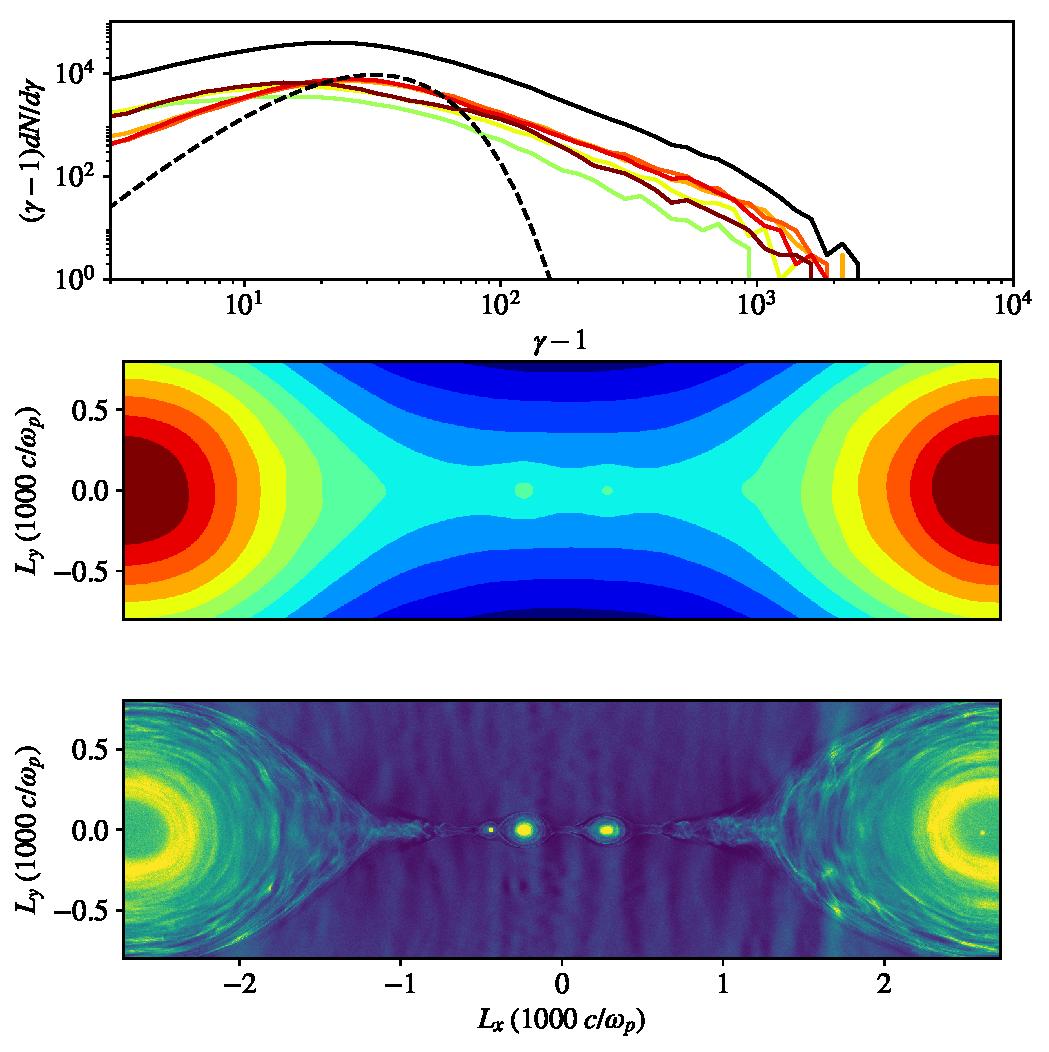
\includegraphics[width =0.5\textwidth]{shellvec_spect2.pdf}
%\caption{Electron energy spectra decomposed into shells around the large magnetic island (top).  The shells are defined by contours of the z-component of the magnetic vector potential (middle).  A spectrum of a given color in the top panel corresponds to particles from the region on the middle panel with the same color.  A Maxwellian is depicted with a dashed black line for reference.  We find that the spectra in every shell has a high energy tail that is much harder than a Maxwellian.  The bottom panel shows a snapshot of the density for reference.}
%\label{shellvec_spect}
%\end{figure}
\begin{figure}[!h]
\centering
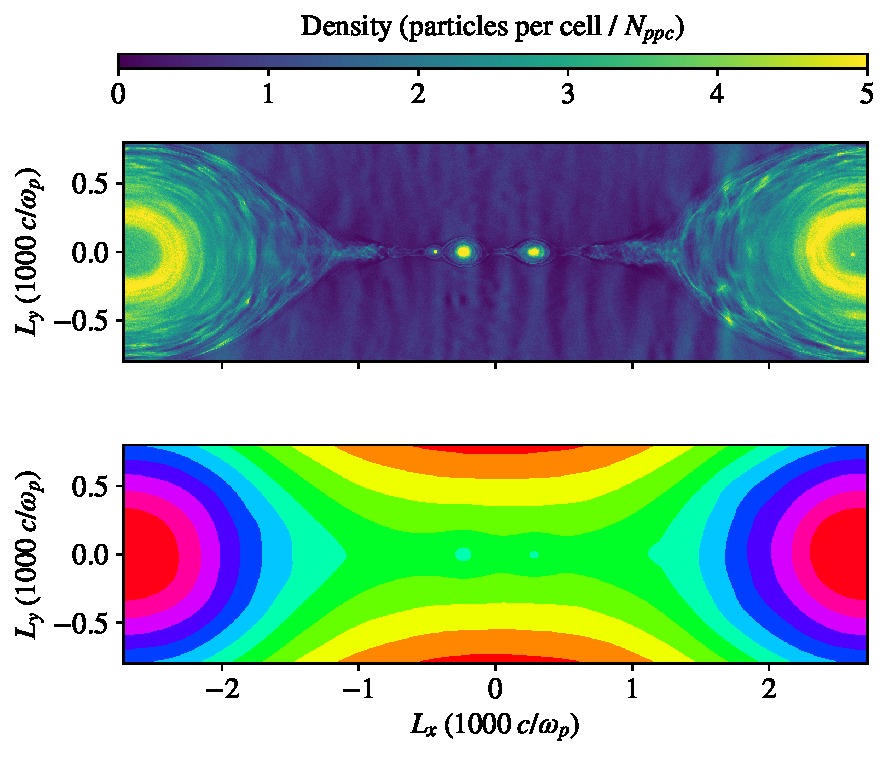
\includegraphics[width =0.75\textwidth]{shellvec_flds.pdf}
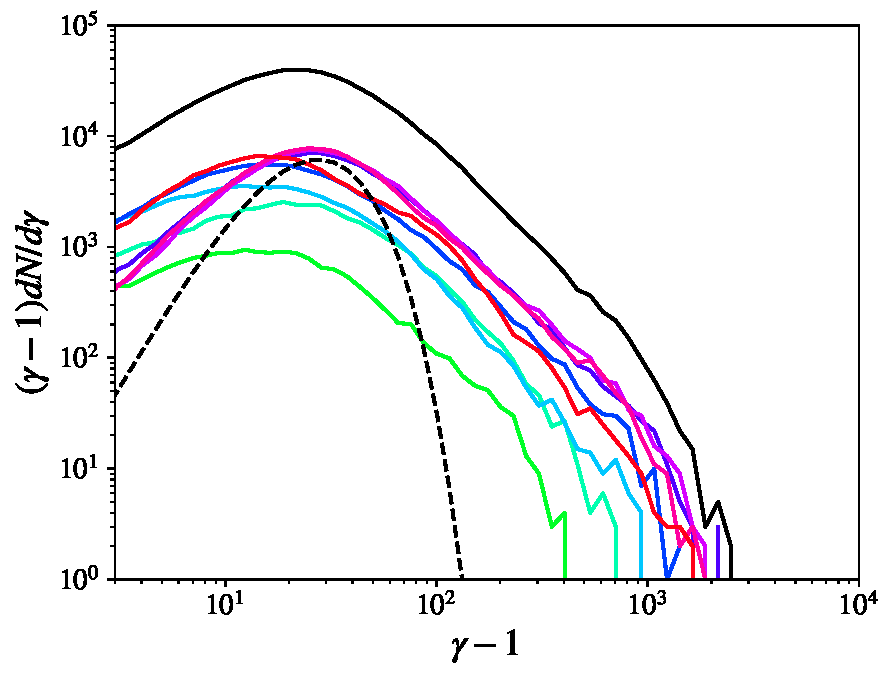
\includegraphics[width =0.75\textwidth]{shellvec_spect.pdf}
\caption{Top: Density profile from a simulation with $\sigma=0.3$, $\beta=0.0003$ (simulation B1), taken at $t\approx 2 t_{A}$.  Middle: Contours of the z-component of the magnetic vector potential.  Bottom: electron spectra decomposed into regions based on the vector potential, colors correspond to the regions in the middle panel.  The solid black line shows the total spectrum and the dashed black line depicts a Maxwellian for reference.}
\label{shellvec_spect}
\end{figure}

